% Options for packages loaded elsewhere
\PassOptionsToPackage{unicode}{hyperref}
\PassOptionsToPackage{hyphens}{url}
%
\documentclass[
]{book}
\usepackage{amsmath,amssymb}
\usepackage{iftex}
\ifPDFTeX
  \usepackage[T1]{fontenc}
  \usepackage[utf8]{inputenc}
  \usepackage{textcomp} % provide euro and other symbols
\else % if luatex or xetex
  \usepackage{unicode-math} % this also loads fontspec
  \defaultfontfeatures{Scale=MatchLowercase}
  \defaultfontfeatures[\rmfamily]{Ligatures=TeX,Scale=1}
\fi
\usepackage{lmodern}
\ifPDFTeX\else
  % xetex/luatex font selection
\fi
% Use upquote if available, for straight quotes in verbatim environments
\IfFileExists{upquote.sty}{\usepackage{upquote}}{}
\IfFileExists{microtype.sty}{% use microtype if available
  \usepackage[]{microtype}
  \UseMicrotypeSet[protrusion]{basicmath} % disable protrusion for tt fonts
}{}
\makeatletter
\@ifundefined{KOMAClassName}{% if non-KOMA class
  \IfFileExists{parskip.sty}{%
    \usepackage{parskip}
  }{% else
    \setlength{\parindent}{0pt}
    \setlength{\parskip}{6pt plus 2pt minus 1pt}}
}{% if KOMA class
  \KOMAoptions{parskip=half}}
\makeatother
\usepackage{xcolor}
\usepackage{color}
\usepackage{fancyvrb}
\newcommand{\VerbBar}{|}
\newcommand{\VERB}{\Verb[commandchars=\\\{\}]}
\DefineVerbatimEnvironment{Highlighting}{Verbatim}{commandchars=\\\{\}}
% Add ',fontsize=\small' for more characters per line
\usepackage{framed}
\definecolor{shadecolor}{RGB}{248,248,248}
\newenvironment{Shaded}{\begin{snugshade}}{\end{snugshade}}
\newcommand{\AlertTok}[1]{\textcolor[rgb]{0.94,0.16,0.16}{#1}}
\newcommand{\AnnotationTok}[1]{\textcolor[rgb]{0.56,0.35,0.01}{\textbf{\textit{#1}}}}
\newcommand{\AttributeTok}[1]{\textcolor[rgb]{0.13,0.29,0.53}{#1}}
\newcommand{\BaseNTok}[1]{\textcolor[rgb]{0.00,0.00,0.81}{#1}}
\newcommand{\BuiltInTok}[1]{#1}
\newcommand{\CharTok}[1]{\textcolor[rgb]{0.31,0.60,0.02}{#1}}
\newcommand{\CommentTok}[1]{\textcolor[rgb]{0.56,0.35,0.01}{\textit{#1}}}
\newcommand{\CommentVarTok}[1]{\textcolor[rgb]{0.56,0.35,0.01}{\textbf{\textit{#1}}}}
\newcommand{\ConstantTok}[1]{\textcolor[rgb]{0.56,0.35,0.01}{#1}}
\newcommand{\ControlFlowTok}[1]{\textcolor[rgb]{0.13,0.29,0.53}{\textbf{#1}}}
\newcommand{\DataTypeTok}[1]{\textcolor[rgb]{0.13,0.29,0.53}{#1}}
\newcommand{\DecValTok}[1]{\textcolor[rgb]{0.00,0.00,0.81}{#1}}
\newcommand{\DocumentationTok}[1]{\textcolor[rgb]{0.56,0.35,0.01}{\textbf{\textit{#1}}}}
\newcommand{\ErrorTok}[1]{\textcolor[rgb]{0.64,0.00,0.00}{\textbf{#1}}}
\newcommand{\ExtensionTok}[1]{#1}
\newcommand{\FloatTok}[1]{\textcolor[rgb]{0.00,0.00,0.81}{#1}}
\newcommand{\FunctionTok}[1]{\textcolor[rgb]{0.13,0.29,0.53}{\textbf{#1}}}
\newcommand{\ImportTok}[1]{#1}
\newcommand{\InformationTok}[1]{\textcolor[rgb]{0.56,0.35,0.01}{\textbf{\textit{#1}}}}
\newcommand{\KeywordTok}[1]{\textcolor[rgb]{0.13,0.29,0.53}{\textbf{#1}}}
\newcommand{\NormalTok}[1]{#1}
\newcommand{\OperatorTok}[1]{\textcolor[rgb]{0.81,0.36,0.00}{\textbf{#1}}}
\newcommand{\OtherTok}[1]{\textcolor[rgb]{0.56,0.35,0.01}{#1}}
\newcommand{\PreprocessorTok}[1]{\textcolor[rgb]{0.56,0.35,0.01}{\textit{#1}}}
\newcommand{\RegionMarkerTok}[1]{#1}
\newcommand{\SpecialCharTok}[1]{\textcolor[rgb]{0.81,0.36,0.00}{\textbf{#1}}}
\newcommand{\SpecialStringTok}[1]{\textcolor[rgb]{0.31,0.60,0.02}{#1}}
\newcommand{\StringTok}[1]{\textcolor[rgb]{0.31,0.60,0.02}{#1}}
\newcommand{\VariableTok}[1]{\textcolor[rgb]{0.00,0.00,0.00}{#1}}
\newcommand{\VerbatimStringTok}[1]{\textcolor[rgb]{0.31,0.60,0.02}{#1}}
\newcommand{\WarningTok}[1]{\textcolor[rgb]{0.56,0.35,0.01}{\textbf{\textit{#1}}}}
\usepackage{longtable,booktabs,array}
\usepackage{calc} % for calculating minipage widths
% Correct order of tables after \paragraph or \subparagraph
\usepackage{etoolbox}
\makeatletter
\patchcmd\longtable{\par}{\if@noskipsec\mbox{}\fi\par}{}{}
\makeatother
% Allow footnotes in longtable head/foot
\IfFileExists{footnotehyper.sty}{\usepackage{footnotehyper}}{\usepackage{footnote}}
\makesavenoteenv{longtable}
\usepackage{graphicx}
\makeatletter
\def\maxwidth{\ifdim\Gin@nat@width>\linewidth\linewidth\else\Gin@nat@width\fi}
\def\maxheight{\ifdim\Gin@nat@height>\textheight\textheight\else\Gin@nat@height\fi}
\makeatother
% Scale images if necessary, so that they will not overflow the page
% margins by default, and it is still possible to overwrite the defaults
% using explicit options in \includegraphics[width, height, ...]{}
\setkeys{Gin}{width=\maxwidth,height=\maxheight,keepaspectratio}
% Set default figure placement to htbp
\makeatletter
\def\fps@figure{htbp}
\makeatother
\setlength{\emergencystretch}{3em} % prevent overfull lines
\providecommand{\tightlist}{%
  \setlength{\itemsep}{0pt}\setlength{\parskip}{0pt}}
\setcounter{secnumdepth}{5}
\usepackage{booktabs}
\ifLuaTeX
  \usepackage{selnolig}  % disable illegal ligatures
\fi
\usepackage[]{natbib}
\bibliographystyle{plainnat}
\usepackage{bookmark}
\IfFileExists{xurl.sty}{\usepackage{xurl}}{} % add URL line breaks if available
\urlstyle{same}
\hypersetup{
  pdftitle={CBW's Bookdown Template Documentation},
  hidelinks,
  pdfcreator={LaTeX via pandoc}}

\title{CBW's Bookdown Template Documentation}
\author{}
\date{\vspace{-2.5em}2024-11-29}

\usepackage{amsthm}
\newtheorem{theorem}{Theorem}[chapter]
\newtheorem{lemma}{Lemma}[chapter]
\newtheorem{corollary}{Corollary}[chapter]
\newtheorem{proposition}{Proposition}[chapter]
\newtheorem{conjecture}{Conjecture}[chapter]
\theoremstyle{definition}
\newtheorem{definition}{Definition}[chapter]
\theoremstyle{definition}
\newtheorem{example}{Example}[chapter]
\theoremstyle{definition}
\newtheorem{exercise}{Exercise}[chapter]
\theoremstyle{definition}
\newtheorem{hypothesis}{Hypothesis}[chapter]
\theoremstyle{remark}
\newtheorem*{remark}{Remark}
\newtheorem*{solution}{Solution}
\begin{document}
\maketitle

{
\setcounter{tocdepth}{1}
\tableofcontents
}
\chapter{CBW's Bookdown Documentation}\label{cbws-bookdown-documentation}

Welcome to CBW's documentation for creating a workshop website using Bookdown. Bookdown is an R package that is used to build books, and in our case, the websites hosting CBW's workshops!

You only need to know markdown and whatever coding language you be using to learn bookdown!

Note, this is the documentation to create a workshop using \emph{bookdown}. If \textbf{Jupyter Book} suits you better, see \href{https://cbw-dev.github.io/jupyterbook-docs/}{here}.

If you don't know which one to use, click \href{}{here} to learn more!

\chapter{Getting Started}\label{getting-started}

Bookdown is an open-source R package that helps write books and articles. We will be building our bookdown-based workshop websites using this, specifically the gitbook template. (This is just the name of the specific template style, you will be working in a workshop template that CBW has prepared for you!)

If you're ready to start making a workshop website in bookdown, let's setup your device (PC, laptop)!

First, let's explain installations.

\section{Installation}\label{installation}

Since bookdown is an R package, you will need R. Plus, our ideal IDE (integrated development environment i.e.~the platform we will be working in) is RStudio.

\begin{enumerate}
\def\labelenumi{\arabic{enumi}.}
\item
  Download and install R (You need R 3.6.0+ installed for RStudio) \href{https://cran.rstudio.com/}{here}. Follow the instructions for your operating system (Linux/macOS/Windows).
  {[}Maybe we should have more installation instructions - a video?{]}
\item
  Download and install RStudio \href{https://posit.co/download/rstudio-desktop/\#:~:text=AND\%20INSTALL\%20R-,2\%3A\%20Install\%20RStudio,-DOWNLOAD\%20RSTUDIO\%20DESKTOP}{here}. Scroll down to find downloads for non-macOS.
\item
  Installl the bookdown R package: Open RStudio and in the console (in the bottom left window of RStudio) run the following command: \texttt{install.packages("bookdown")}
\end{enumerate}

We're ready to start working with CBW's bookdown workshop template now!

\chapter{\texorpdfstring{Starting to Set Up Your \textbf{New} Workshop}{Starting to Set Up Your New Workshop}}\label{starting-to-set-up-your-new-workshop}

Certain aspects of the setup for workshops will be different depending on your role. Headers ending in ``(RC)'' are for Regional Coordinators. Headers without ``(RC)'' are assumed to be relevant to both RC and workshop teams.

\section{Workshop Setup (RC)}\label{workshop-setup-rc}

Regional Coordinators will be tasked with creating and slightly editing each new repository for each new workshop.

\begin{enumerate}
\def\labelenumi{\arabic{enumi}.}
\item
  First, let's go the \href{https://github.com/cbw-dev/bookdown-template}{bookdown template}.
\item
  Click on the ``Use this template'' green button, which is to the left of the title of the repository ``bookdown-template''. Then, press the dropdown option: ``Create a new repository'', as seen below.
\end{enumerate}

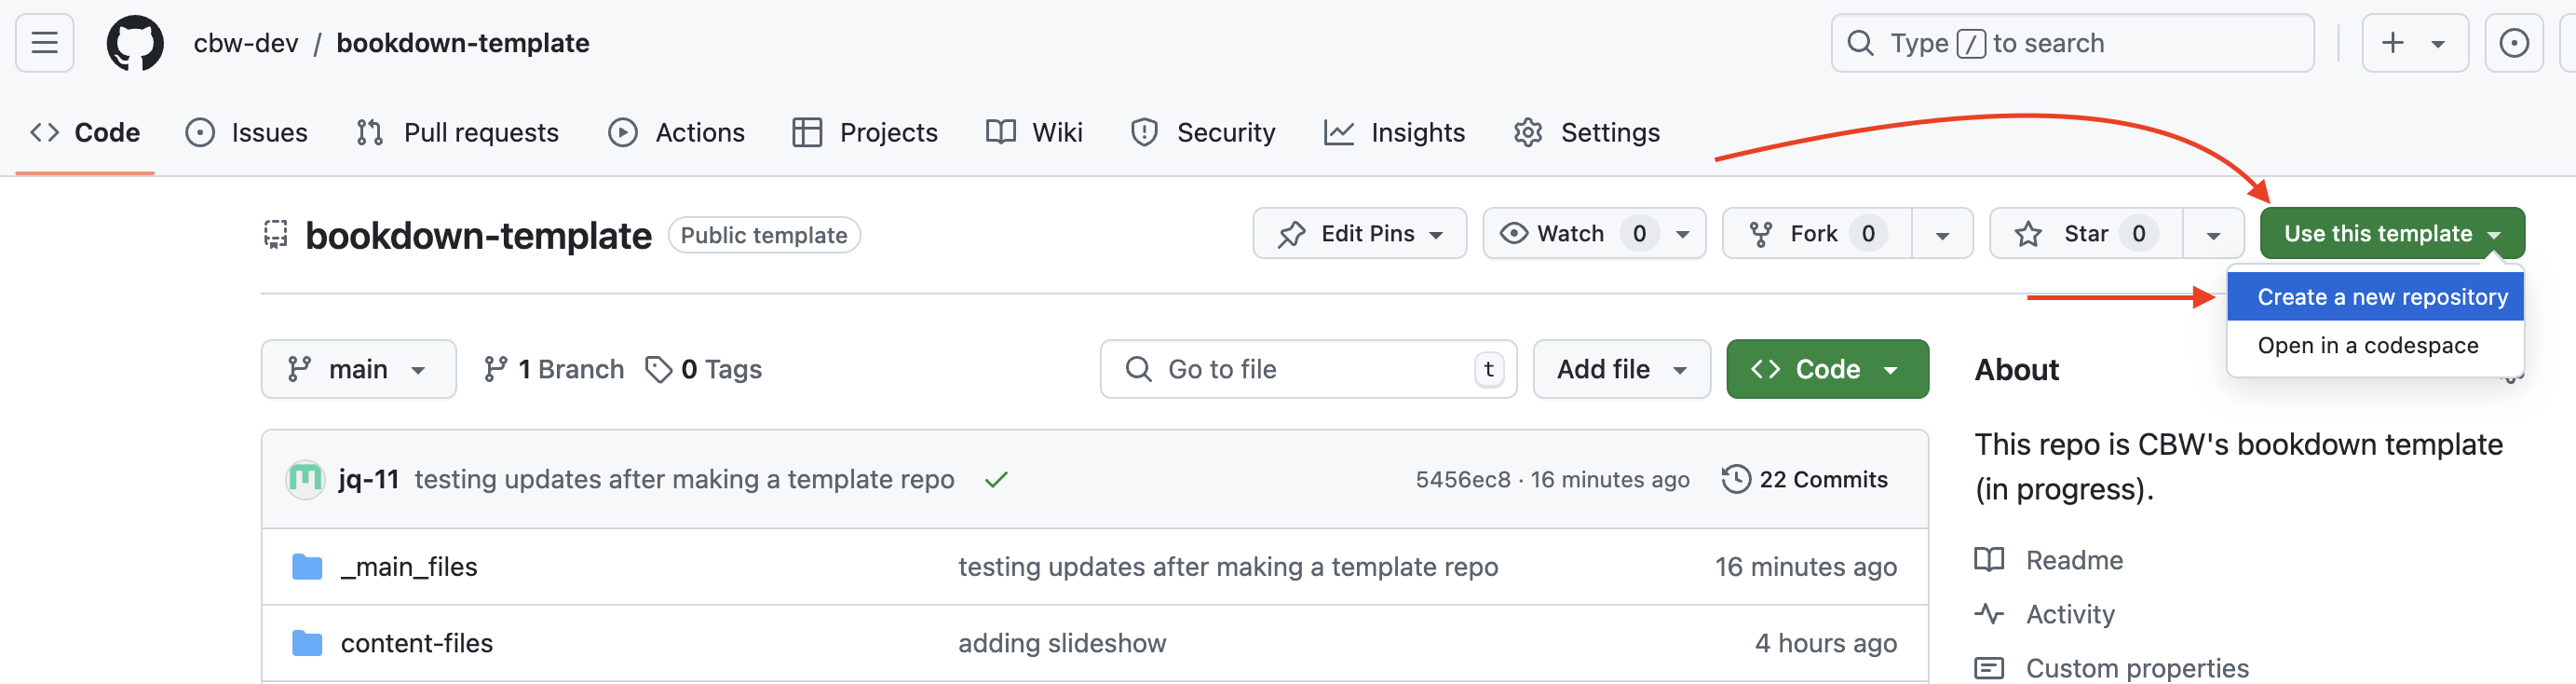
\includegraphics{img/template/make-a-template.png}\\

\begin{enumerate}
\def\labelenumi{\arabic{enumi}.}
\setcounter{enumi}{2}
\tightlist
\item
  You will be brought to a ``Create a new repository'' page. Fill out the blanks as seen below. That is, change the owner to XXX, make it public, fill in the repository name and description according to \href{}{CBW Guidelines}. ``Include all branches'' does not need to be selected (???).
\end{enumerate}

NOTE: CHANGE OWNER TO XXX (ask Nia, probably cbw-dev for now)
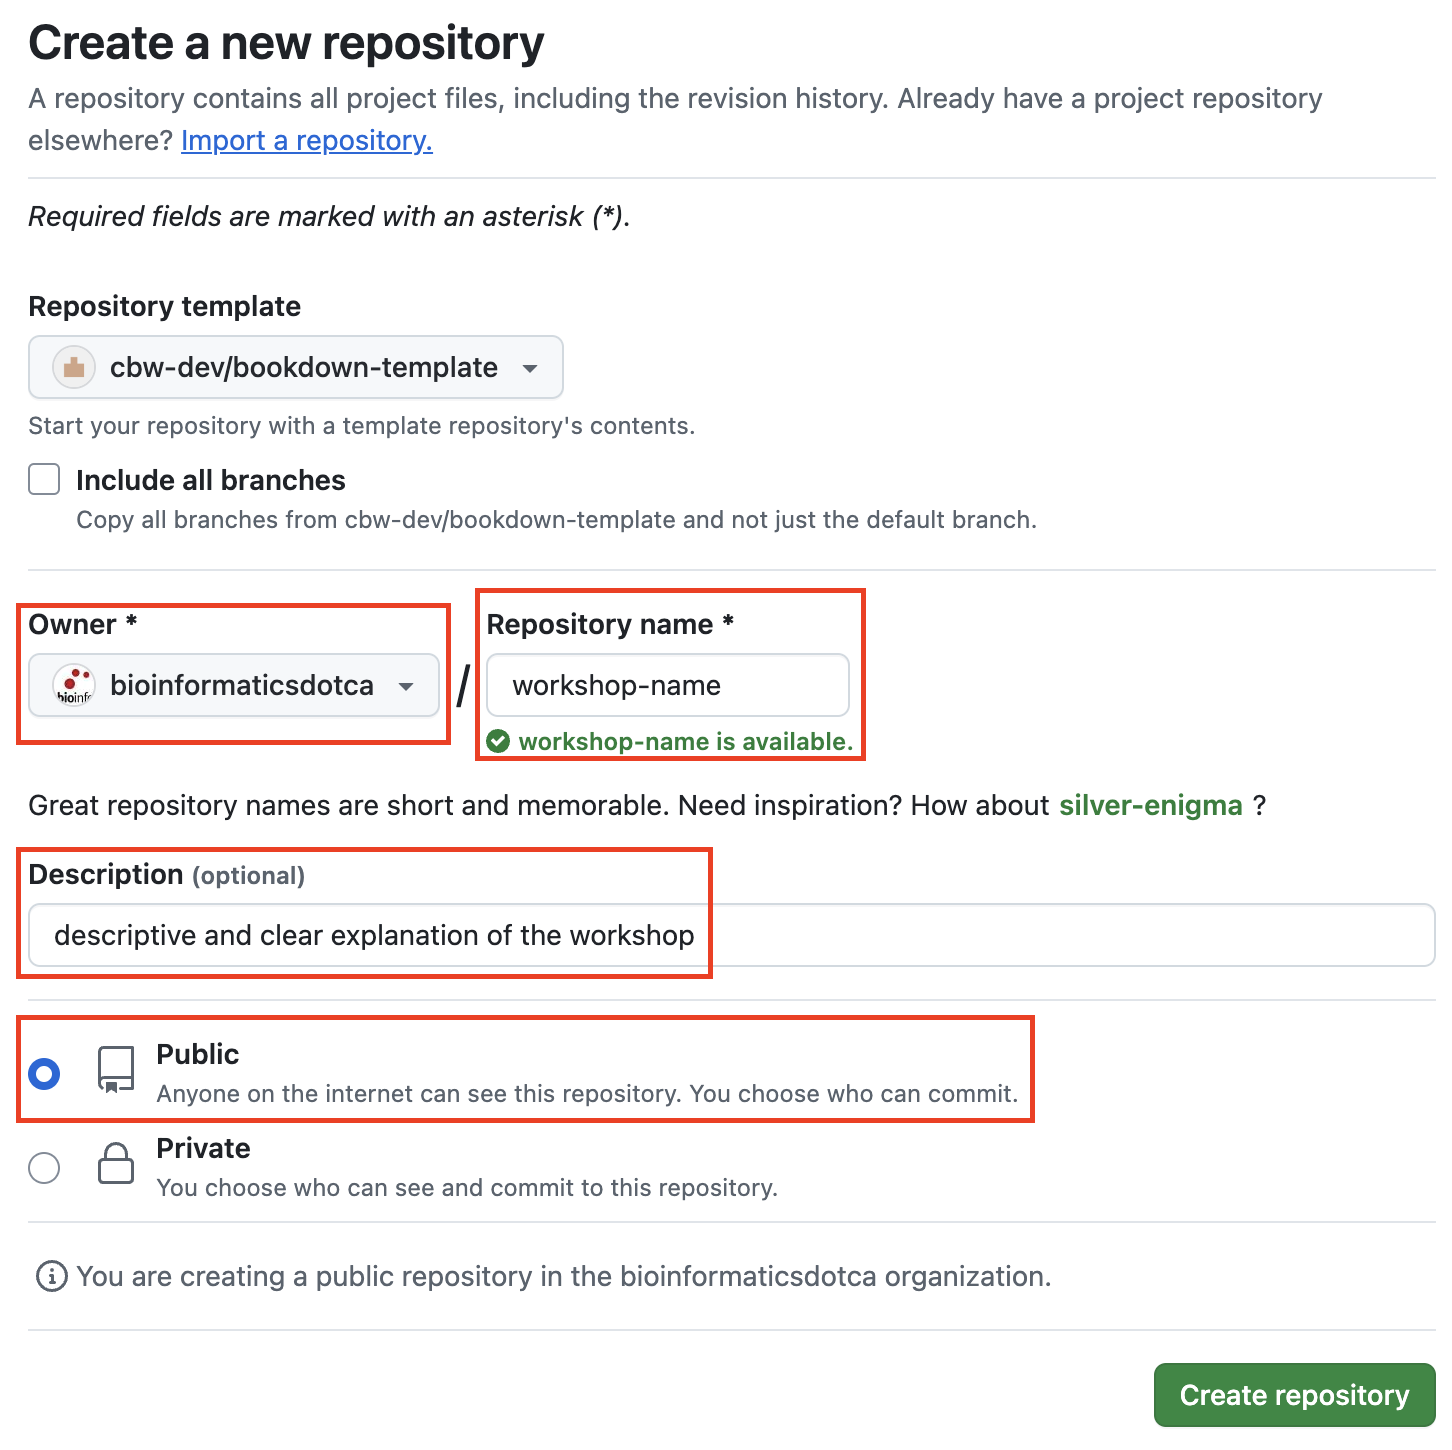
\includegraphics{img/template/make-new-repo.png}\\

This may take a couple seconds to generate. After it loads, you will be brought to a new repository for the new workshop!

Now, let's turn this into a website - let's deploy!

\subsection{How to Deploy Your Workshop Website}\label{how-to-deploy-your-workshop-website}

\begin{enumerate}
\def\labelenumi{\arabic{enumi}.}
\item
  In the top navigation bar, select settings.
  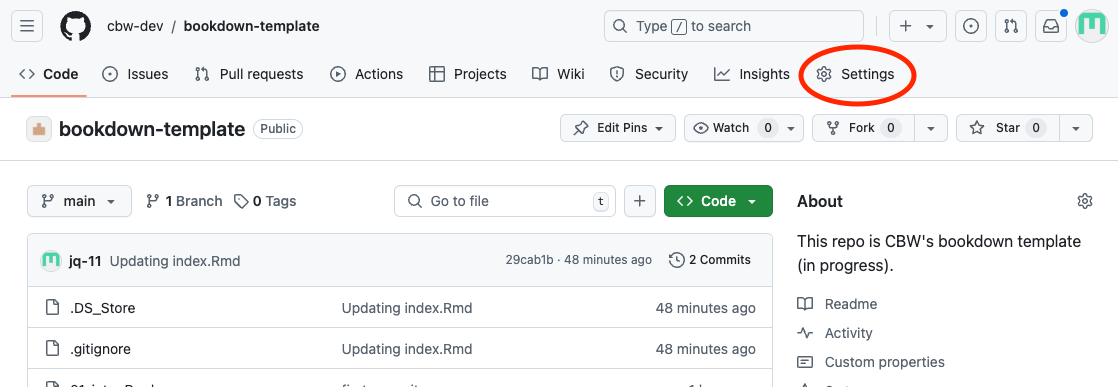
\includegraphics{img/git-instruct/github-settings.png}
\item
  Then, go to the pages sidebar.
  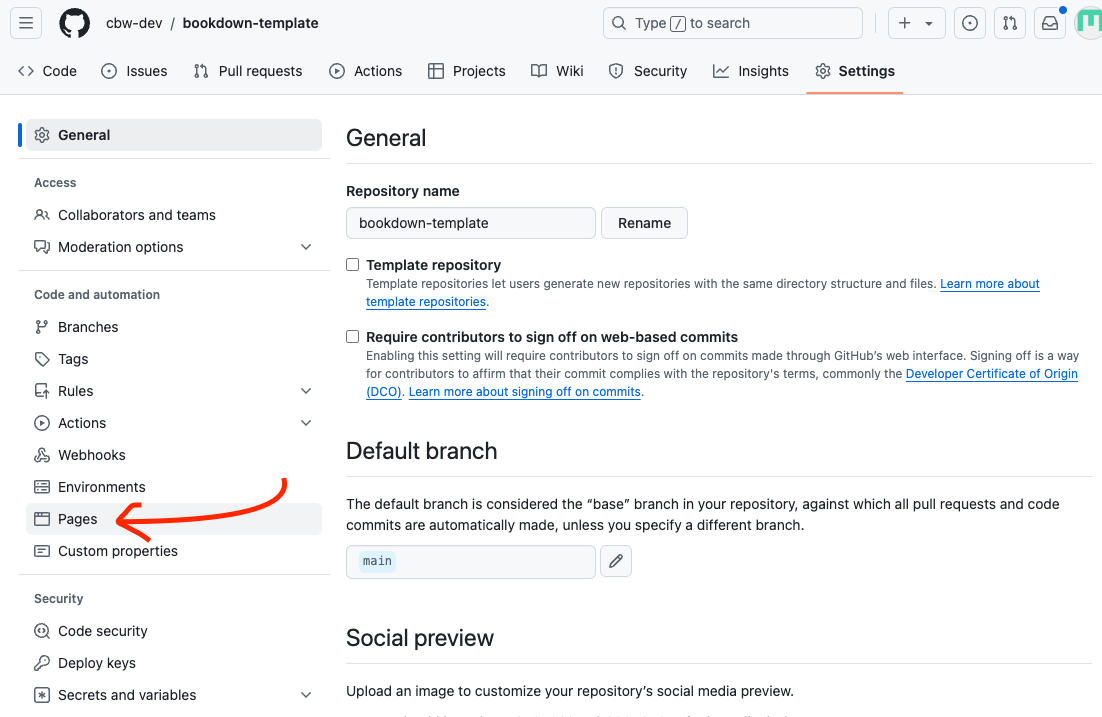
\includegraphics{img/git-instruct/github-select-pages.png}
\item
  ``Deploy from a branch'' is already selected, which is what we want. We must change the branch from ``none'' to main.
  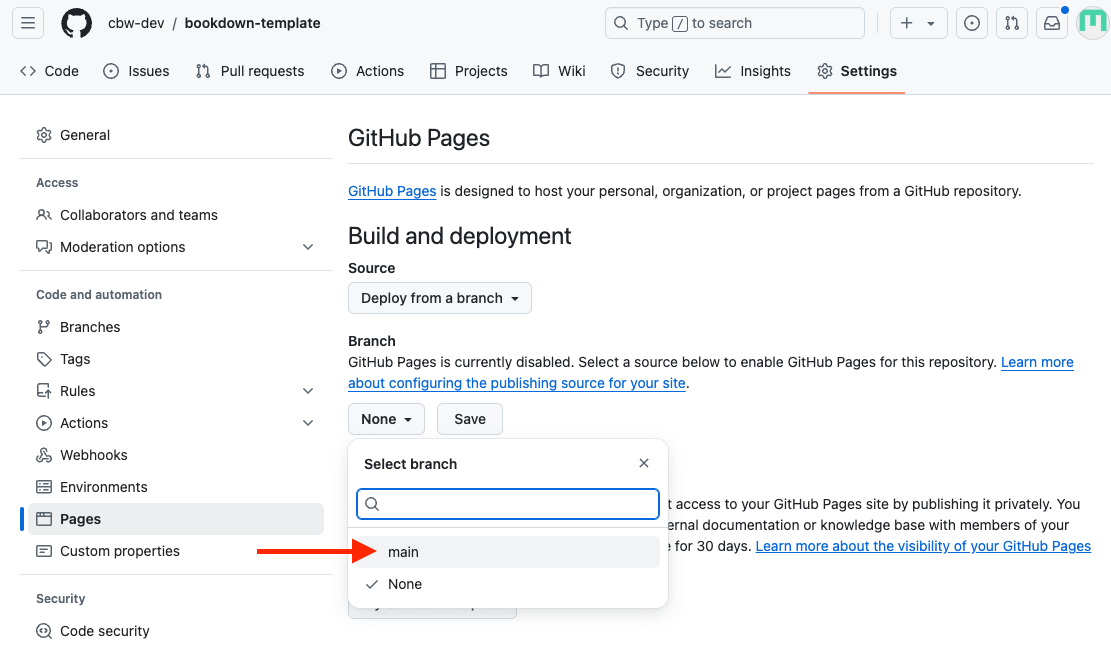
\includegraphics{img/git-instruct/github-deploy-main.png}
\item
  Then, change the folder from \texttt{/\ root} to \texttt{/docs}. Then press save.
  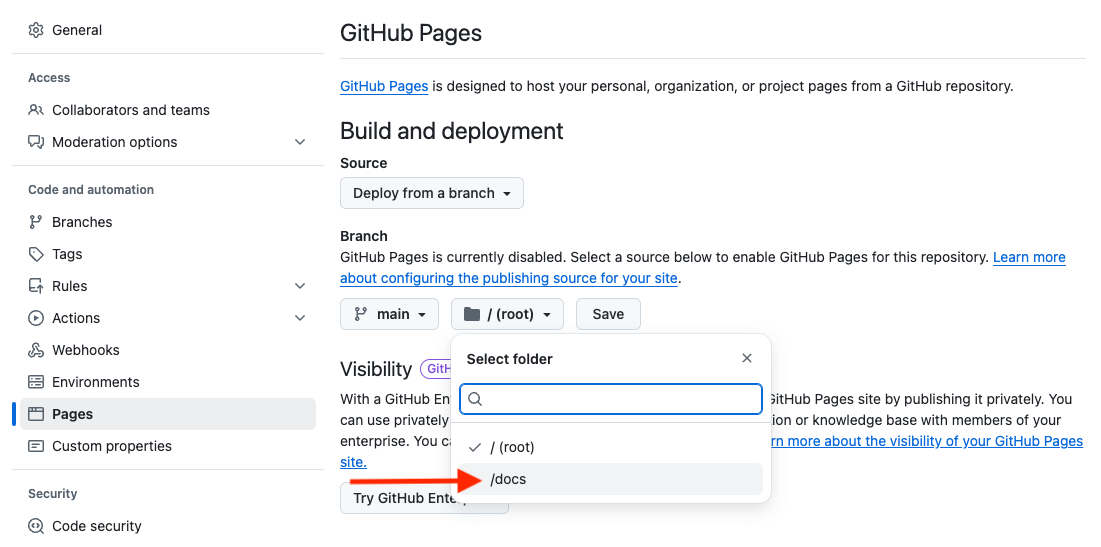
\includegraphics{img/git-instruct/github-deploy-docs.png}\\
\end{enumerate}

Great! Now we're waiting on the page to build and deploy, which should take less than a minute.

To see updates, go to the \textbf{Actions} page (found along the top navigation bar. This will help you understand how the deploy is working, and if it succeeded or failed.

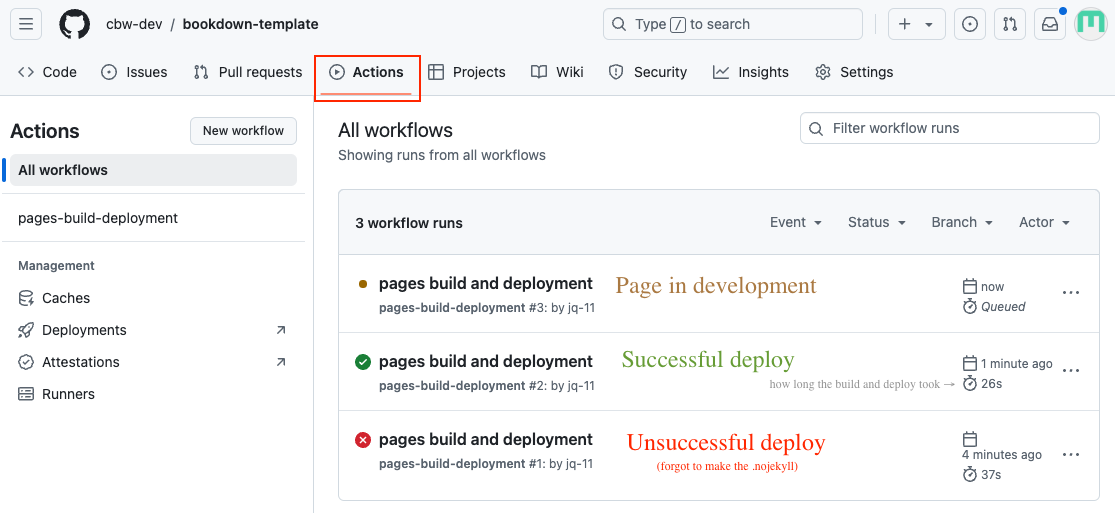
\includegraphics{img/git-instruct/github-pages-actions-explained.png}\\

You can click \textbf{pages build and deployment} for updates. It will give you errors (which may not be very clear) or the link of your deployed page!

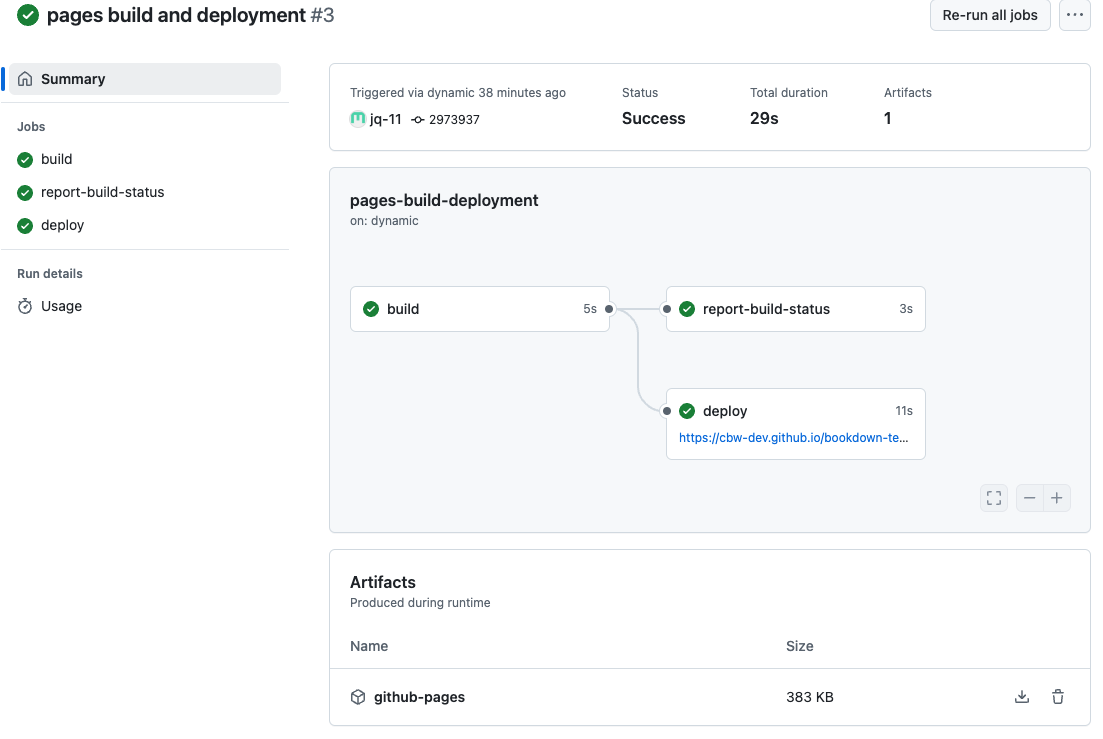
\includegraphics{img/git-instruct/successful-deploy.png}\\
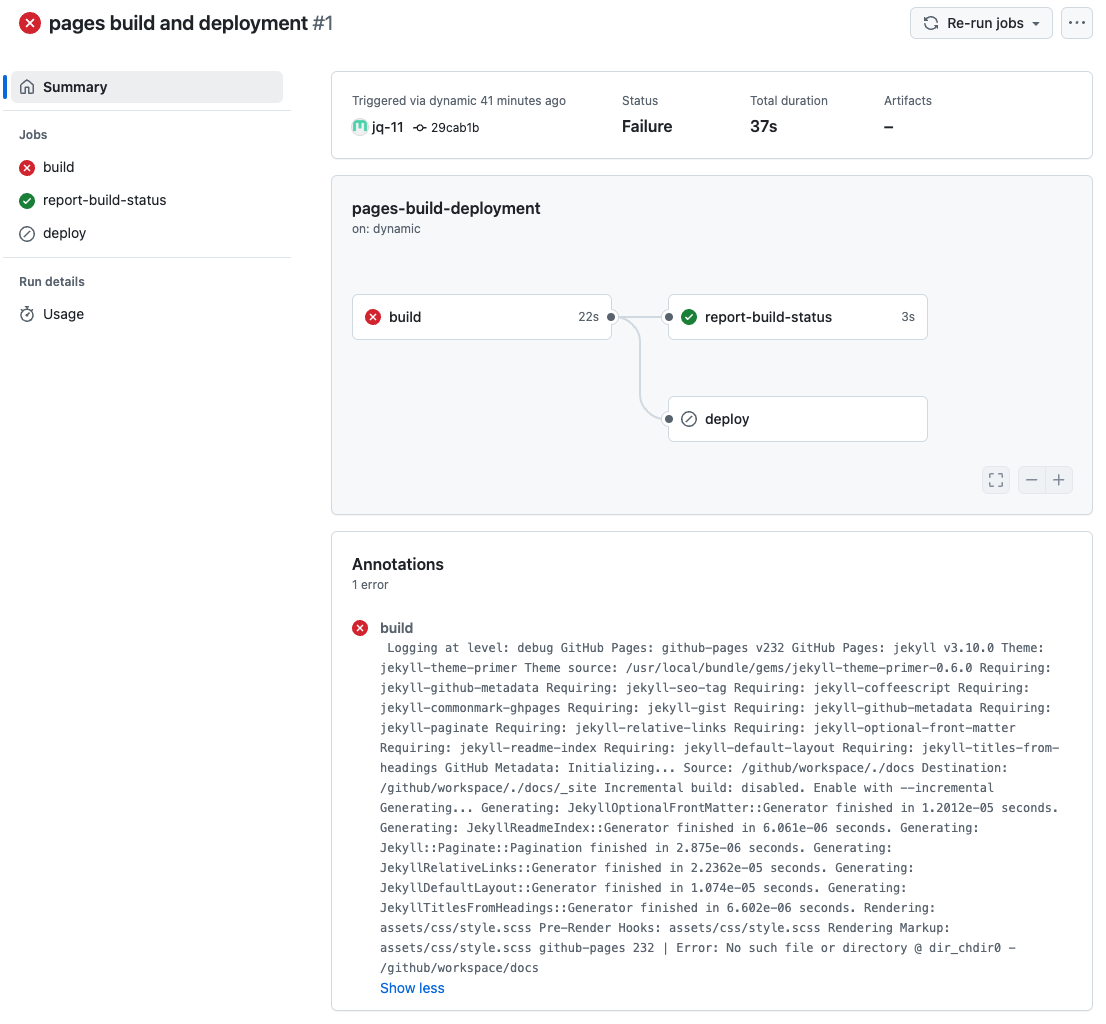
\includegraphics{img/git-instruct/failed-deploy.png}\\

\section{Setting Up Team Access (Nia will fill this in)}\label{setting-up-team-access-nia-will-fill-this-in}

\section{Getting the Template on Your Local Computer - Git Clone}\label{getting-the-template-on-your-local-computer---git-clone}

\begin{enumerate}
\def\labelenumi{\arabic{enumi}.}
\item
  navigate to where in your local file system you want to have your workshop in (hint: cd)
\item
  git clone \href{mailto:git@github.com}{\nolinkurl{git@github.com}}:jq-11/workshop-name.git
\item
  ready to go ! you should have permissions to git push
\end{enumerate}

\begin{quote}
NOTE: Consider having only one team member (or perhaps your RC) make git pushes or control pull requests. To avoid merge conflicts, designate 1 team member to control actual changes to your workshop repo. Other team members can fork or create branches, and create a pull request that the designated team member can check and overlook.
\end{quote}

But what do any of these files mean? Which ones do I edit? Which ones shouldn't I edit? How do I open this in RStudio? It's time for you to go to the next page :D

\chapter{So What Do These Files Mean?}\label{so-what-do-these-files-mean}

Ok now we all have our workshop locally, which is made up of all these files and folders?

First, let's figure out RStudio. Skip to \hyperref[file-setup]{file setup} if you already know how to use RStudio (and it's built in git control window).

\section{Open in RStudio}\label{open-in-rstudio}

Enter the folder you just git cloned, it should be titled ``{[}workshop-name{]}''. Right click on {[}workshop-name{]}.Rproj and press ``Open in RStudio''. There is only one file with this file ending.

A RStudio window should open up and look like the image below.
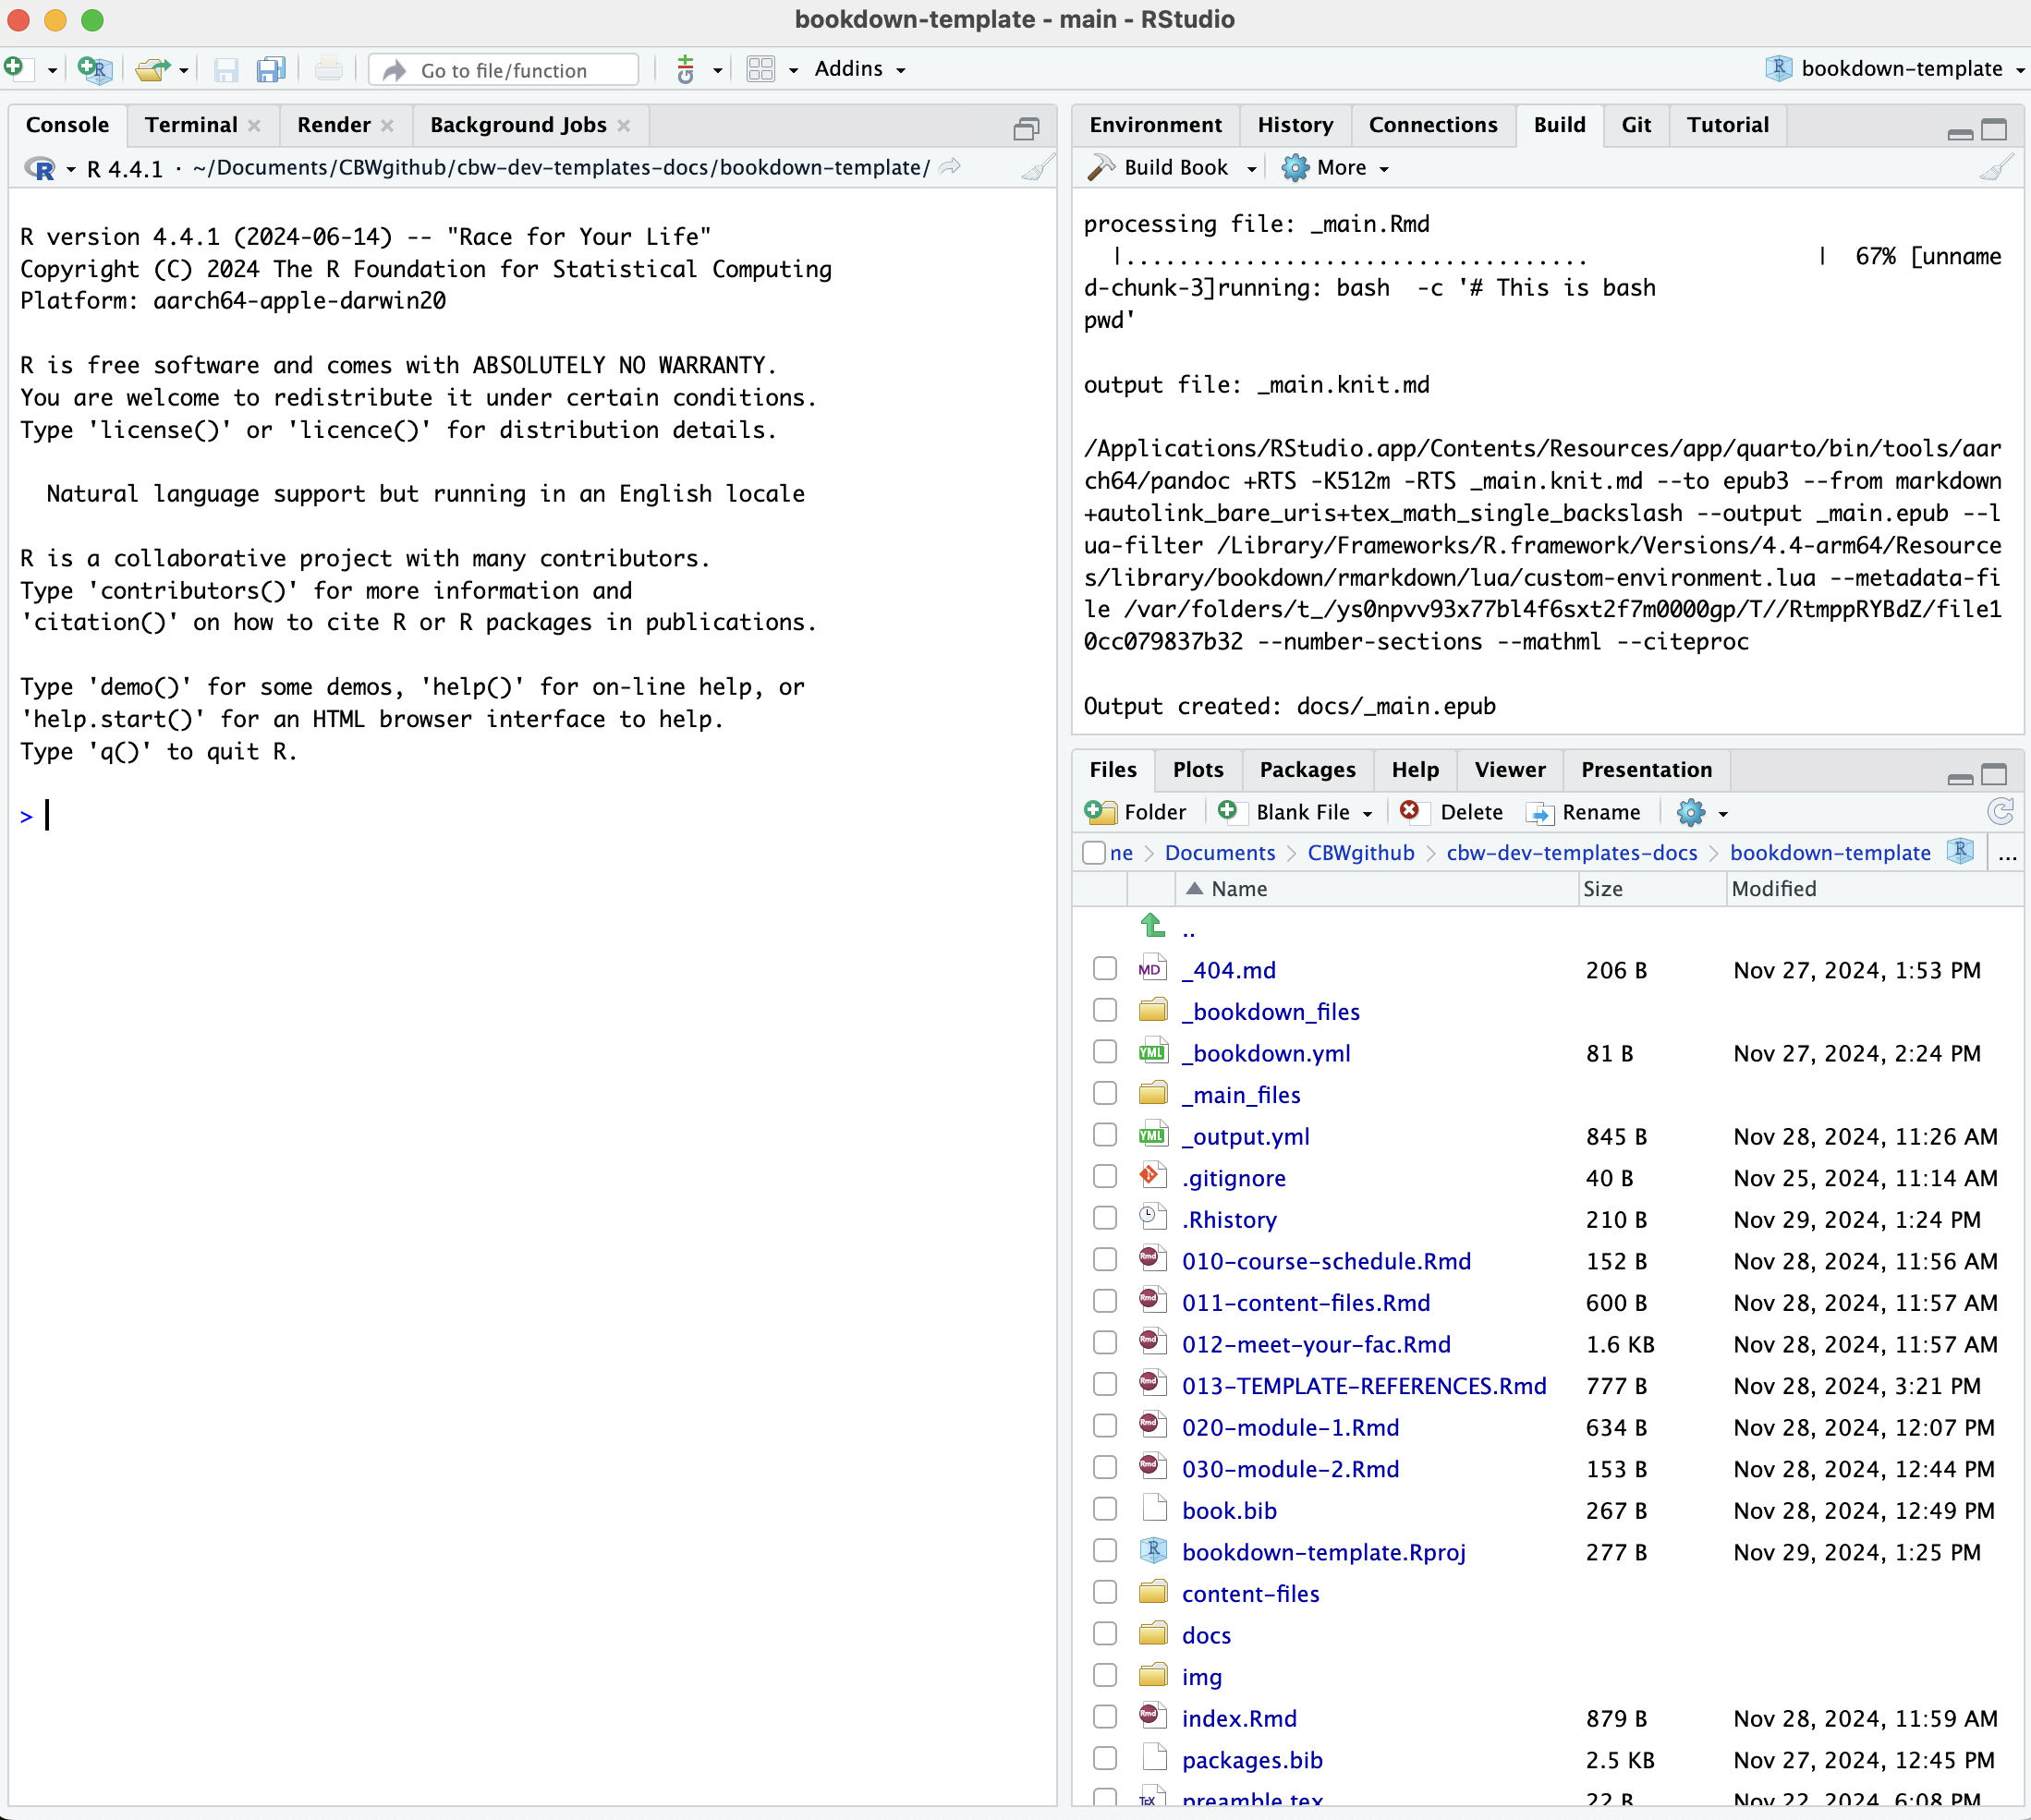
\includegraphics{img/files-and-build/newly-opened-RStudio.png}\\

\section{Explaining RStudio}\label{explaining-rstudio}

In the bottom left, have our console and other debug related windows (such as terminal!). Any code we run will appear in the console. We can access the terminal (just like editing in the Terminal app) under the ``Terminal'' tab.

In the bottom right, we have all of our files and subfolders. These files will be explained \hyperref[file-setup]{below}. This window also contains helpful views, like ``Viewer'' and ``Plots''. We will touch on these later.

Try opening \texttt{index.Rmd}: a new pane will open in the top left that shows the contents of \texttt{index.Rmd}. This is where we will be editing our files! Notice, the ``Knit'' button.

In your top right, we have a different window with more different views. The most relevant windows to us are the ``Build'' and the ``Git'' windows.

\begin{quote}
No ``Git'' Window?

Try closing (and maybe even restarting RStudio) and then reopening it. A ``Git'' tab should appear to the right of the ``Build'' tab and to the left of the ``Tutorial'' tab.
\end{quote}

\section{Build the book}\label{build-the-book}

Try pressing ``Build Book'' within the ``Build'' window. Your build window is going to fill up with text, and soon, a website is going to pop-up as your new window. This is the website you will be editing to create your workshop!

By building the book, all of these files were compiled and converted to .html files, that create a website. Each time we make local changes to our files and we want them to appear in our website, we need to rebuild the book. Note that each time we build our book, the files we edited will be saved first (we don't have to save before building!).

\subsection{Other Ways to Build Your Book}\label{other-ways-to-build-your-book}

\begin{enumerate}
\def\labelenumi{\arabic{enumi}.}
\tightlist
\item
  Build the book from the R console:
\end{enumerate}

\begin{Shaded}
\begin{Highlighting}[]
\NormalTok{bookdown}\SpecialCharTok{::}\FunctionTok{render\_book}\NormalTok{()}
\end{Highlighting}
\end{Shaded}

\begin{enumerate}
\def\labelenumi{\arabic{enumi}.}
\setcounter{enumi}{1}
\tightlist
\item
  Press the keyboard buttons: \texttt{cmd\ OR\ ctrl\ +\ shift\ +\ B}
\end{enumerate}

\subsection{Knit Your Book}\label{knit-your-book}

Building can take a long time. If you are editing just one file, you can press the ``Knit'' button that is at the top of the window with your file. This will run the code in the page, and show you what that page would look like in the website (as well as saving that file).

\begin{quote}
Note: Other pages in your website will not update.
\end{quote}

\begin{quote}
A quicker way to knit is using the keboard controls

\texttt{cmd\ OR\ ctrl\ +\ shift\ +\ K}
\end{quote}

\subsection{Preview Your Book}\label{preview-your-book}

If you want live updates to your changes, you can preview the page as you edit the book when you save individual .Rmd files. You can start the server in a work session by using the RStudio add-in ``Preview book'', or from the R console (in the bottom left window):

\begin{Shaded}
\begin{Highlighting}[]
\NormalTok{bookdown}\SpecialCharTok{::}\FunctionTok{serve\_book}\NormalTok{()}
\end{Highlighting}
\end{Shaded}

But which files do we edit? Well alas, it's time to discuss the file setup.

\section{File Setup Explanation}\label{file-setup}

Explain file setup (tree diagram?)

\section{Push Your Changes}\label{push-your-changes}

\chapter{Storing all formatting content}\label{storing-all-formatting-content}

\begin{itemize}
\tightlist
\item
  How to edit index.Rmd
\end{itemize}

\section{Chapters}\label{chapters}

All chapters start with a first-level heading followed by your chapter title, like the line above. There should be only one first-level heading (\texttt{\#}) per .Rmd file.

\section{A section}\label{a-section}

All chapter sections start with a second-level (\texttt{\#\#}) or higher heading followed by your section title, like the sections above and below here. You can have as many as you want within a chapter.

\subsection*{An unnumbered section}\label{an-unnumbered-section}
\addcontentsline{toc}{subsection}{An unnumbered section}

Chapters and sections are numbered by default. To un-number a heading, add a \texttt{\{.unnumbered\}} or the shorter \texttt{\{-\}} at the end of the heading, like in this section.

\section{Cross-references}\label{cross}

Cross-references make it easier for your readers to find and link to elements in your book.

\section{Chapters and sub-chapters}\label{chapters-and-sub-chapters}

There are two steps to cross-reference any heading:

\begin{enumerate}
\def\labelenumi{\arabic{enumi}.}
\tightlist
\item
  Label the heading: \texttt{\#\ Hello\ world\ \{\#nice-label\}}.

  \begin{itemize}
  \tightlist
  \item
    Leave the label off if you like the automated heading generated based on your heading title: for example, \texttt{\#\ Hello\ world} = \texttt{\#\ Hello\ world\ \{\#hello-world\}}.
  \item
    To label an un-numbered heading, use: \texttt{\#\ Hello\ world\ \{-\#nice-label\}} or \texttt{\{\#\ Hello\ world\ .unnumbered\}}.
  \end{itemize}
\item
  Next, reference the labeled heading anywhere in the text using \texttt{\textbackslash{}@ref(nice-label)}; for example, please see Chapter \ref{cross}.

  \begin{itemize}
  \tightlist
  \item
    If you prefer text as the link instead of a numbered reference use: \hyperref[cross]{any text you want can go here}.
  \end{itemize}
\end{enumerate}

\section{Captioned figures and tables}\label{captioned-figures-and-tables}

Figures and tables \emph{with captions} can also be cross-referenced from elsewhere in your book using \texttt{\textbackslash{}@ref(fig:chunk-label)} and \texttt{\textbackslash{}@ref(tab:chunk-label)}, respectively.

See Figure \ref{fig:nice-fig}.

\begin{Shaded}
\begin{Highlighting}[]
\FunctionTok{par}\NormalTok{(}\AttributeTok{mar =} \FunctionTok{c}\NormalTok{(}\DecValTok{4}\NormalTok{, }\DecValTok{4}\NormalTok{, .}\DecValTok{1}\NormalTok{, .}\DecValTok{1}\NormalTok{))}
\FunctionTok{plot}\NormalTok{(pressure, }\AttributeTok{type =} \StringTok{\textquotesingle{}b\textquotesingle{}}\NormalTok{, }\AttributeTok{pch =} \DecValTok{19}\NormalTok{)}
\end{Highlighting}
\end{Shaded}

\begin{figure}

{\centering 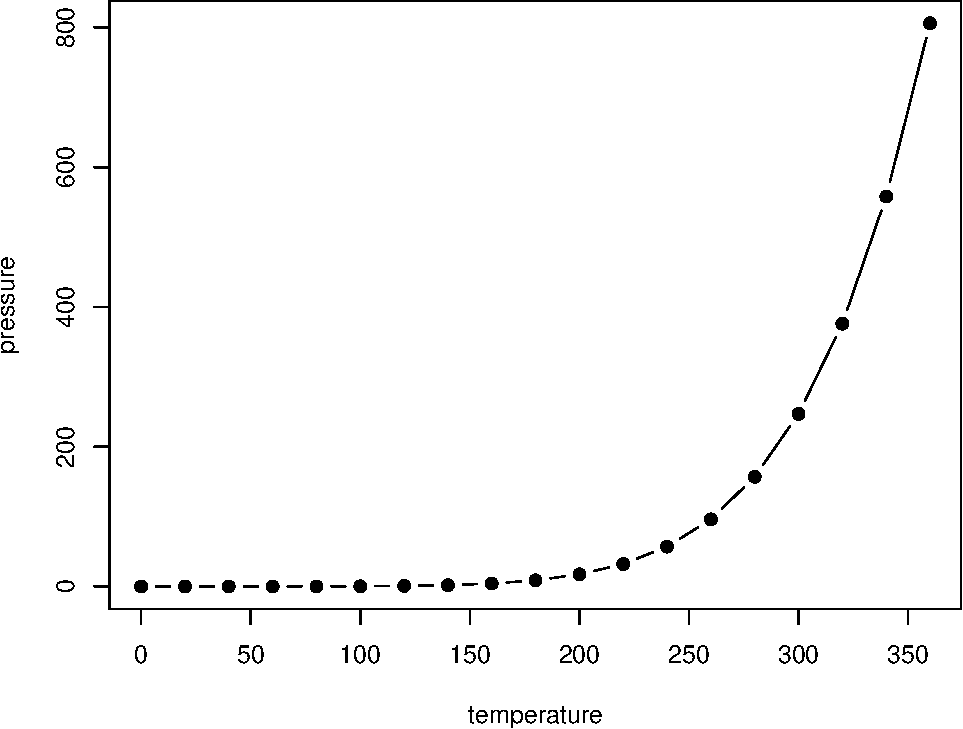
\includegraphics[width=0.8\linewidth]{_main_files/figure-latex/nice-fig-1} 

}

\caption{Here is a nice figure!}\label{fig:nice-fig}
\end{figure}

Don't miss Table \ref{tab:nice-tab}.

\begin{Shaded}
\begin{Highlighting}[]
\NormalTok{knitr}\SpecialCharTok{::}\FunctionTok{kable}\NormalTok{(}
  \FunctionTok{head}\NormalTok{(pressure, }\DecValTok{10}\NormalTok{), }\AttributeTok{caption =} \StringTok{\textquotesingle{}Here is a nice table!\textquotesingle{}}\NormalTok{,}
  \AttributeTok{booktabs =} \ConstantTok{TRUE}
\NormalTok{)}
\end{Highlighting}
\end{Shaded}

\begin{table}

\caption{\label{tab:nice-tab}Here is a nice table!}
\centering
\begin{tabular}[t]{rr}
\toprule
temperature & pressure\\
\midrule
0 & 0.0002\\
20 & 0.0012\\
40 & 0.0060\\
60 & 0.0300\\
80 & 0.0900\\
\addlinespace
100 & 0.2700\\
120 & 0.7500\\
140 & 1.8500\\
160 & 4.2000\\
180 & 8.8000\\
\bottomrule
\end{tabular}
\end{table}

\section{Parts}\label{parts}

You can add parts to organize one or more book chapters together. Parts can be inserted at the top of an .Rmd file, before the first-level chapter heading in that same file.

Add a numbered part: \texttt{\#\ (PART)\ Act\ one\ \{-\}} (followed by \texttt{\#\ A\ chapter})

Add an unnumbered part: \texttt{\#\ (PART\textbackslash{}*)\ Act\ one\ \{-\}} (followed by \texttt{\#\ A\ chapter})

Add an appendix as a special kind of un-numbered part: \texttt{\#\ (APPENDIX)\ Other\ stuff\ \{-\}} (followed by \texttt{\#\ A\ chapter}). Chapters in an appendix are prepended with letters instead of numbers.

\section{Footnotes}\label{footnotes}

Footnotes are put inside the square brackets after a caret \texttt{\^{}{[}{]}}. Like this one \footnote{This is a footnote.}.

\section{Citations}\label{citations}

Reference items in your bibliography file(s) using \texttt{@key}.

For example, we are using the \textbf{bookdown} package \citep{R-bookdown} (check out the last code chunk in index.Rmd to see how this citation key was added) in this sample book, which was built on top of R Markdown and \textbf{knitr} \citep{xie2015} (this citation was added manually in an external file book.bib).
Note that the \texttt{.bib} files need to be listed in the index.Rmd with the YAML \texttt{bibliography} key.

The RStudio Visual Markdown Editor can also make it easier to insert citations: \url{https://rstudio.github.io/visual-markdown-editing/\#/citations}

\section{Blocks}\label{blocks}

\section{Equations}\label{equations}

Here is an equation.

\begin{equation} 
  f\left(k\right) = \binom{n}{k} p^k\left(1-p\right)^{n-k}
  \label{eq:binom}
\end{equation}

You may refer to using \texttt{\textbackslash{}@ref(eq:binom)}, like see Equation \eqref{eq:binom}.

\section{Theorems and proofs}\label{theorems-and-proofs}

Labeled theorems can be referenced in text using \texttt{\textbackslash{}@ref(thm:tri)}, for example, check out this smart theorem \ref{thm:tri}.

\begin{theorem}
\protect\hypertarget{thm:tri}{}\label{thm:tri}For a right triangle, if \(c\) denotes the \emph{length} of the hypotenuse
and \(a\) and \(b\) denote the lengths of the \textbf{other} two sides, we have
\[a^2 + b^2 = c^2\]
\end{theorem}

Read more here \url{https://bookdown.org/yihui/bookdown/markdown-extensions-by-bookdown.html}.

\section{Callout blocks}\label{callout-blocks}

The R Markdown Cookbook provides more help on how to use custom blocks to design your own callouts: \url{https://bookdown.org/yihui/rmarkdown-cookbook/custom-blocks.html}

\section{Sharing your book}\label{sharing-your-book}

\section{Publishing}\label{publishing}

HTML books can be published online, see: \url{https://bookdown.org/yihui/bookdown/publishing.html}

\section{404 pages}\label{pages}

By default, users will be directed to a 404 page if they try to access a webpage that cannot be found. If you'd like to customize your 404 page instead of using the default, you may add either a \texttt{\_404.Rmd} or \texttt{\_404.md} file to your project root and use code and/or Markdown syntax.

\section{Metadata for sharing}\label{metadata-for-sharing}

Bookdown HTML books will provide HTML metadata for social sharing on platforms like Twitter, Facebook, and LinkedIn, using information you provide in the \texttt{index.Rmd} YAML. To setup, set the \texttt{url} for your book and the path to your \texttt{cover-image} file. Your book's \texttt{title} and \texttt{description} are also used.

This \texttt{gitbook} uses the same social sharing data across all chapters in your book- all links shared will look the same.

Specify your book's source repository on GitHub using the \texttt{edit} key under the configuration options in the \texttt{\_output.yml} file, which allows users to suggest an edit by linking to a chapter's source file.

Read more about the features of this output format here:

\url{https://pkgs.rstudio.com/bookdown/reference/gitbook.html}

Or use:

\begin{Shaded}
\begin{Highlighting}[]
\NormalTok{?bookdown}\SpecialCharTok{::}\NormalTok{gitbook}
\end{Highlighting}
\end{Shaded}

\chapter{How to Render Code}\label{how-to-render-code}

\chapter{Brain Dump / FAQ}\label{brain-dump-faq}

\section{Danger Zones}\label{danger-zones}

\begin{itemize}
\item
  renaming your file with this project, doesn't change the .Rprog file!
\item
  GIT TIPS PAGE ???
\item
  BEST PRACTICES PAGE
\item
  MAKE SURE TO EXPLAIN WHAT HAPPENS WHEN MERGE CONFLICTS APPEAR
\end{itemize}

Ex. Forgot to pull before editing?
- Your git window will say (at the top of the window) your branch is ahead of the main branch
- You will probably have to deal with a merge conflict
- {[}this is pretty in-depth{]}

\begin{itemize}
\tightlist
\item
  update favicon.ico image in template with one with higher quality
\end{itemize}

\section{Potential Errors \& Bugs}\label{potential-errors-bugs}

\begin{itemize}
\item
  If you get a bug where your website builds into a website that looks like it is made using very simple html, you may have to change your permissions. If you see \textbf{``Permission denied''} in your warning messages, trying running this command \texttt{chmod\ -R\ u+w\ docs} in terminal, in the folder containing your docs folder {[}CLARIFY ?{]}
\item
  \textbf{``Could not produce X output''} - by default, bookdown builds all possible formats: gitbook, pdf, epub versions. We only need the gitbook, so if you're having issues, change your build settings to only creating the gitbook {[}CLARIFY + INCLUDE IMAGES{]}
\item
  A very common bug is \textbf{``missing X package''}, just install it using this command in your console (the bottom left window in RStudio) \texttt{install.packages("missing\ package\ name,\ include\ these\ surrouding\ quotations")}
\end{itemize}

\section{FAQ}\label{faq}

\part{DEVELOPERS GUIDE}\label{part-developers-guide}

\chapter{Build Site}\label{build-site}

\section{How to edit \_bookdown.yml}\label{how-to-edit-_bookdown.yml}

\begin{itemize}
\tightlist
\item
  add a new line, \texttt{output\_dir:\ "docs"} to \_bookdown.yml
\item
  build the site
\item
  add a \texttt{.nojekyll} file into the produced docs folder
\end{itemize}

\section{How to edit \_output.yml (RC)}\label{how-to-edit-_output.yml-rc}

\begin{itemize}
\tightlist
\item
  after \emph{before:} change your workshop name link
\item
  after \emph{edit:} put the link to the workshop repo, and end the link with \texttt{/\%s}
\item
  save
\end{itemize}

\section{Mandatory ``index.Rmd'' landing page}\label{mandatory-index.rmd-landing-page}

Each \textbf{bookdown} chapter is an .Rmd file, and each .Rmd file can contain one (and only one) chapter. A chapter \emph{must} start with a first-level heading: \texttt{\#\ A\ good\ chapter}, and can contain one (and only one) first-level heading.

Use second-level and higher headings within chapters like: \texttt{\#\#\ A\ short\ section} or \texttt{\#\#\#\ An\ even\ shorter\ section}.

The \texttt{index.Rmd} file is required, and is also your first book chapter. It will be the homepage when you render the book.

\section{Build the book:}\label{build-the-book-1}

\begin{itemize}
\tightlist
\item
  ``Build'' button in RStudio IDE /OR/ bookdown::render\_book()
\item
  Preview the book: - updates on saves in viewer window bookdown::serve\_book()
\end{itemize}

Before building

\subsection{Render book}\label{render-book}

You can render the HTML version of this example book without changing anything:

\begin{enumerate}
\def\labelenumi{\arabic{enumi}.}
\item
  Find the \textbf{Build} pane in the RStudio IDE, and
\item
  Click on \textbf{Build Book}, then select your output format, or select ``All formats'' if you'd like to use multiple formats from the same book source files.
\end{enumerate}

Or build the book from the R console:

\begin{Shaded}
\begin{Highlighting}[]
\NormalTok{bookdown}\SpecialCharTok{::}\FunctionTok{render\_book}\NormalTok{()}
\end{Highlighting}
\end{Shaded}

To render this example to PDF as a \texttt{bookdown::pdf\_book}, you'll need to install XeLaTeX. You are recommended to install TinyTeX (which includes XeLaTeX): \url{https://yihui.org/tinytex/}.

\subsection{Preview book}\label{preview-book}

As you work, you may start a local server to live preview this HTML book. This preview will update as you edit the book when you save individual .Rmd files. You can start the server in a work session by using the RStudio add-in ``Preview book'', or from the R console:

\begin{Shaded}
\begin{Highlighting}[]
\NormalTok{bookdown}\SpecialCharTok{::}\FunctionTok{serve\_book}\NormalTok{()}
\end{Highlighting}
\end{Shaded}

\chapter{Git Instructions}\label{git-instructions}

\section{How to Make a Git Repo (RC)}\label{how-to-make-a-git-repo-rc}

\begin{enumerate}
\def\labelenumi{\arabic{enumi}.}
\item
  Go to \url{https://github.com/cbw-dev} (CHANGE?) and scroll to your repositories.
\item
  Click the green ``New'' button to the right of the repositories search bar.
\item
  Create the new repository. Give it a \emph{name} and \emph{description}. Select \emph{Public} instead of private, as shown below.
\end{enumerate}

\begin{quote}
🚧 Warning

MAKE NAMING CONVENTION
\end{quote}

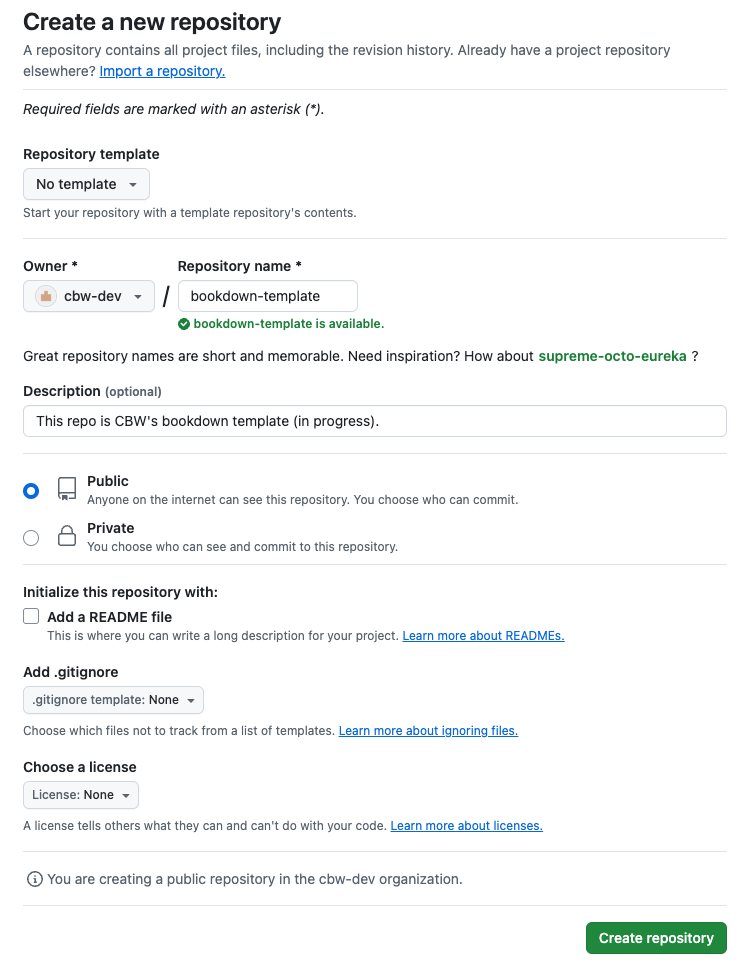
\includegraphics{img/git-instruct/create-git-repo.png}
4. Click the green \emph{Create repository} button at the bottom.

Now, we already have a local project. Now we want it on GitHub, so everyone on your team can make changes to the workshop! Let's make the GitHub connection (i.e let's add our local code to GitHub!)

\subsection{How to Make the Git Connection (Adding your Local Repo to GitHub)}\label{how-to-make-the-git-connection-adding-your-local-repo-to-github}

After the previous step, you will be brought to this page.The only things that will differ are the name of the repo.

\begin{figure}
\centering
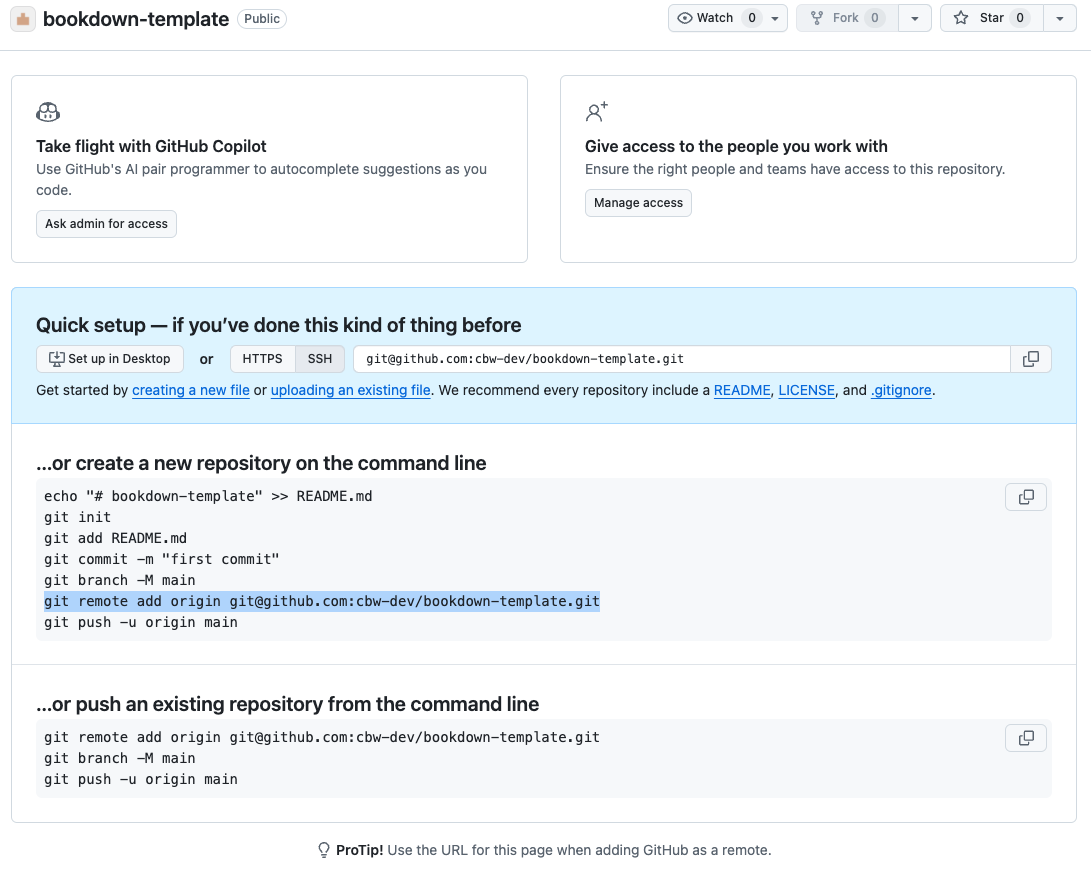
\includegraphics{img/git-instruct/git-connection.png}
\caption{landing page after making a git repo}
\end{figure}

\begin{enumerate}
\def\labelenumi{\arabic{enumi}.}
\setcounter{enumi}{4}
\item
  Open Terminal (Mac) or Command Prompt/Powershell (Windows).
\item
  Go to where we created the bookdown project.
\item
  Once inside the folder with the project. Let's make the git repo. First we initialize: \texttt{git\ init}. (Put this into terminal and press enter.)
\item
  Let's add all the files: \texttt{git\ add\ *}
\item
  Let's commit these files, with a descriptive message to help make it clear to others what we just did. For now, our message can be simple: \texttt{git\ commit\ -m\ "first\ commit"}. (Put this into terminal and press enter.)
\item
  Next, put this into terminal and press enter: \texttt{git\ branch\ -M\ main}.
\item
  \textbf{Important:} This step is why I highlighted that specific text above. Copy that command, and put it into terminal. Generally, it will look something like this: \texttt{git\ remote\ add\ origin\ git@github.com:cbw-dev/NAME-OF-YOUR-REPO.git}
\item
  Next, put \texttt{git\ push\ -u\ origin\ main} into terminal and press enter.
\end{enumerate}

All the steps are shown below.

\begin{figure}
\centering
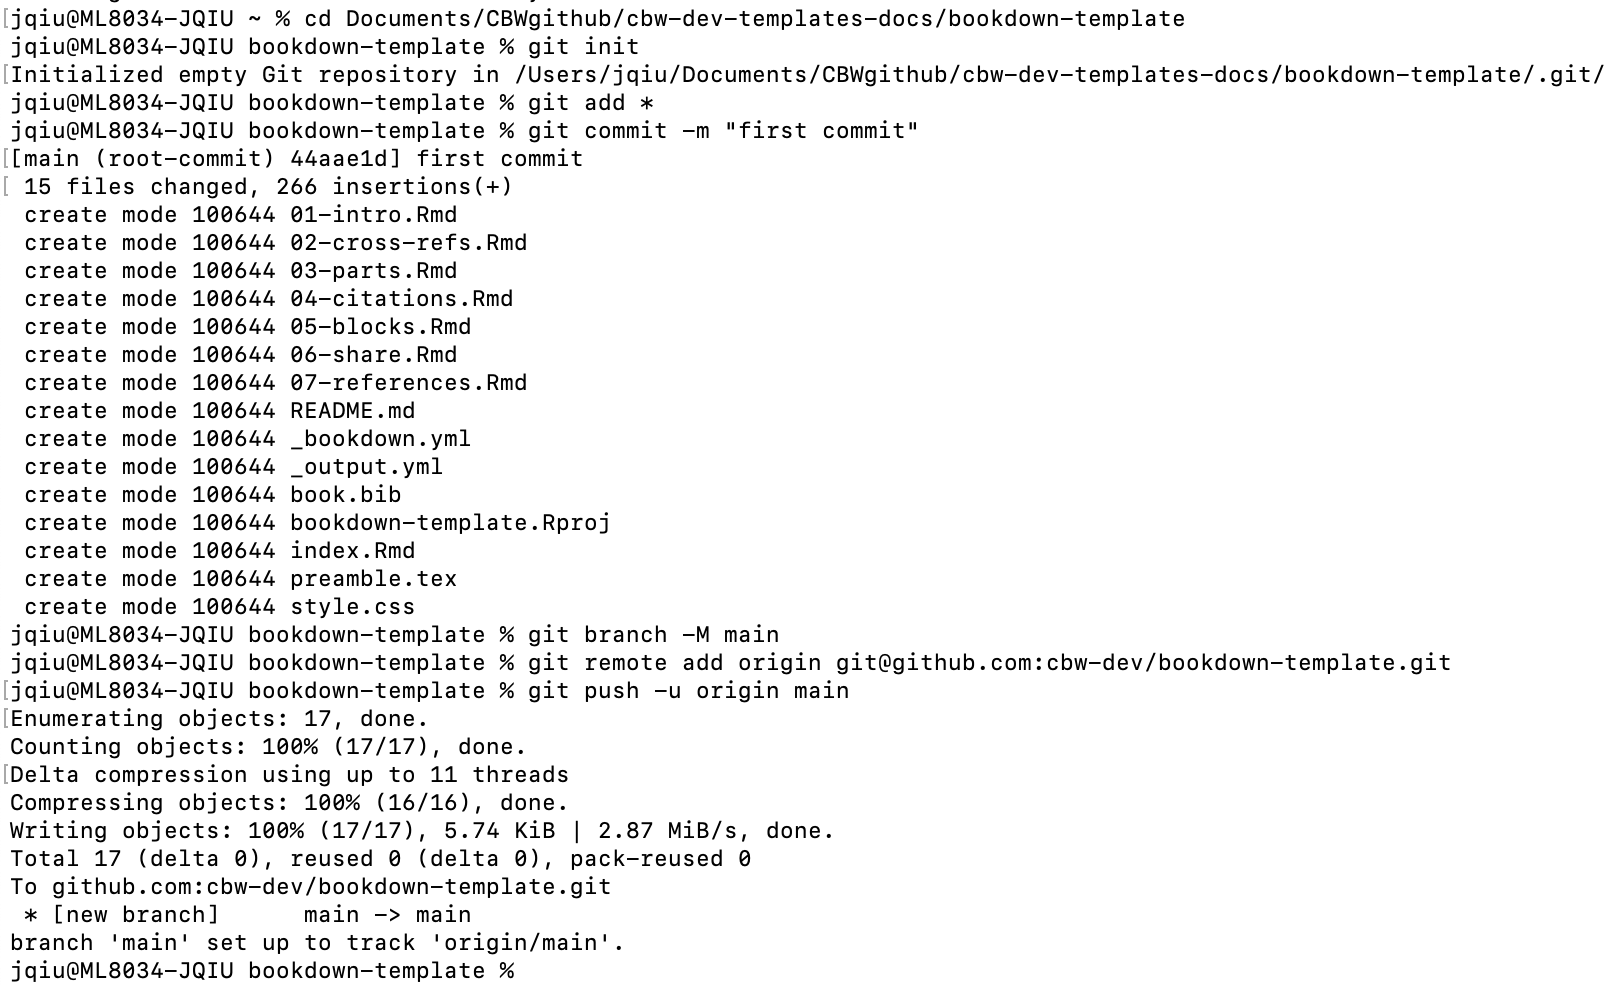
\includegraphics{img/git-instruct/git-instructions-in-terminal.png}
\caption{all the git steps typed out into terminal with results}
\end{figure}

\section{Updating GitHub via RStudio}\label{updating-github-via-rstudio}

Now, close your RStudio session, and reopen it.

Now, we will be able to see a Git window in the top right. Click ``Git'' to open this window.

\begin{figure}
\centering
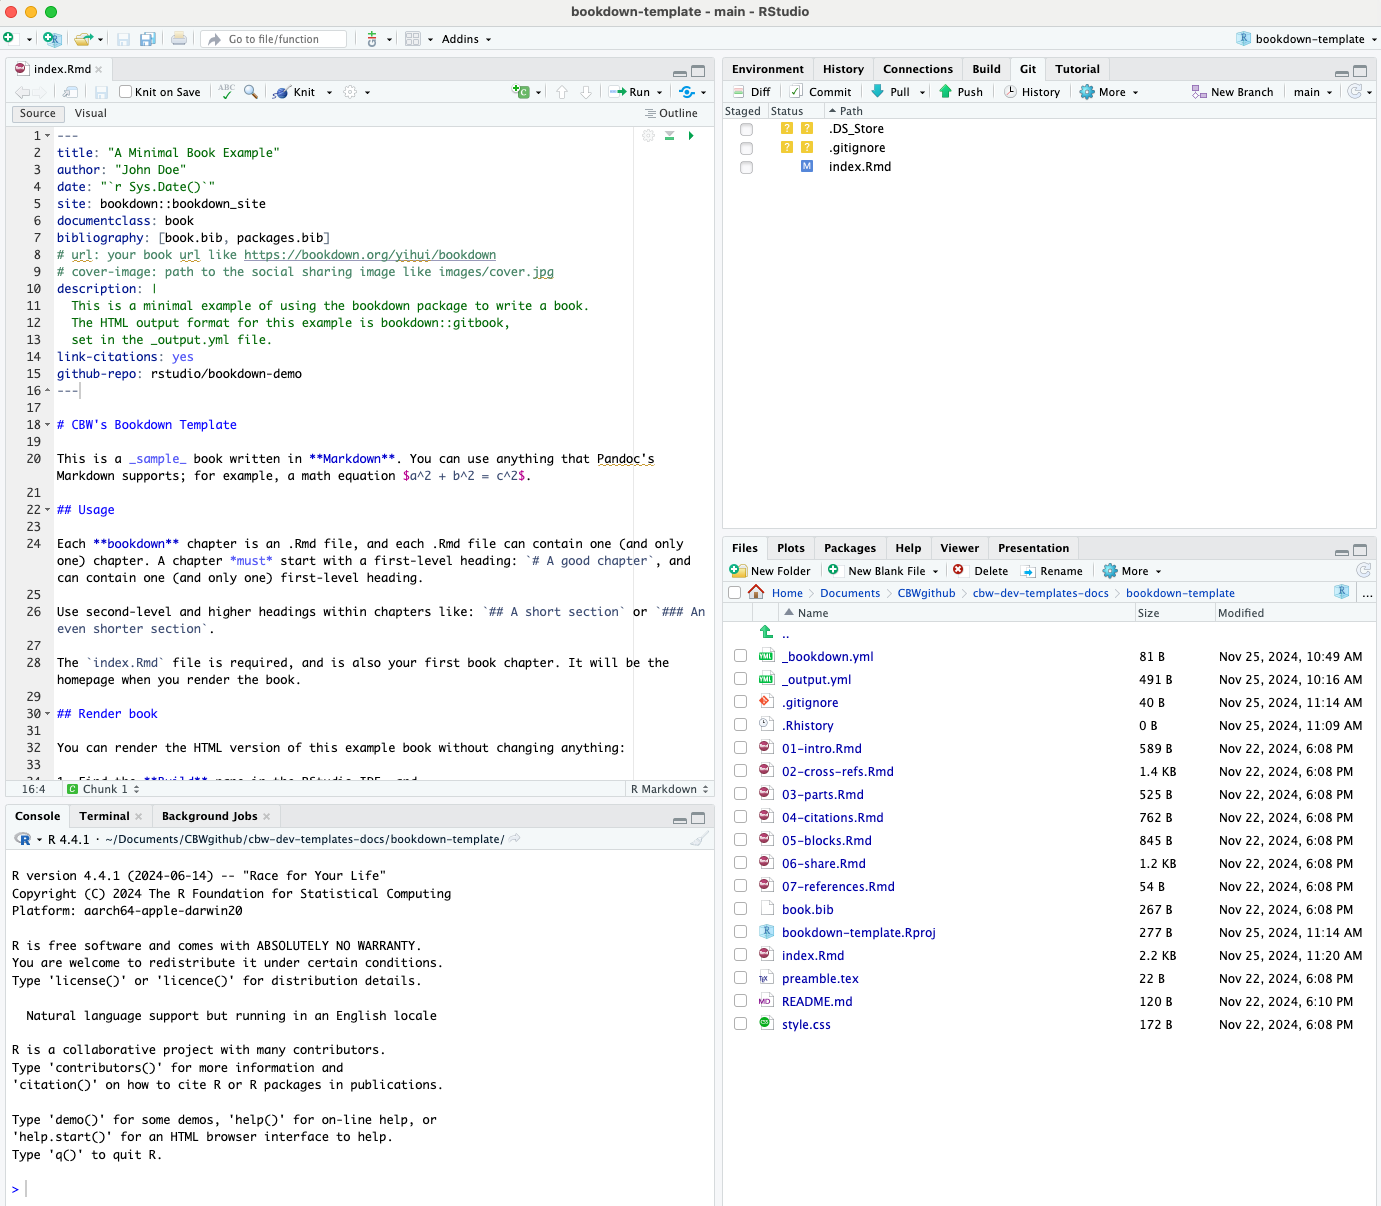
\includegraphics{img/git-instruct/RStudio-with-git-window-open.png}
\caption{RStudio with Git window open}
\end{figure}

Let's say we only edited \texttt{index.Rmd}, now we see the newly edited files. (Do not worry too much about \texttt{.DS\_Store} and \texttt{.gitignore} do.) Let's try to push this change to GitHub.

\begin{enumerate}
\def\labelenumi{\arabic{enumi}.}
\setcounter{enumi}{12}
\tightlist
\item
  Select all the edited files.
\end{enumerate}

\begin{figure}
\centering
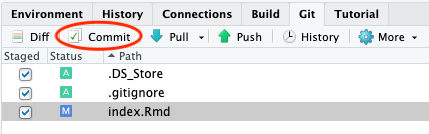
\includegraphics{img/git-instruct/git-window-selected-items.png}
\caption{selected files in the git window and the commit button highlighted}
\end{figure}

\begin{enumerate}
\def\labelenumi{\arabic{enumi}.}
\setcounter{enumi}{13}
\tightlist
\item
  Then, click the Commit button, which appears above your selected items. A window pane will appear (shown below).
\end{enumerate}

\begin{figure}
\centering
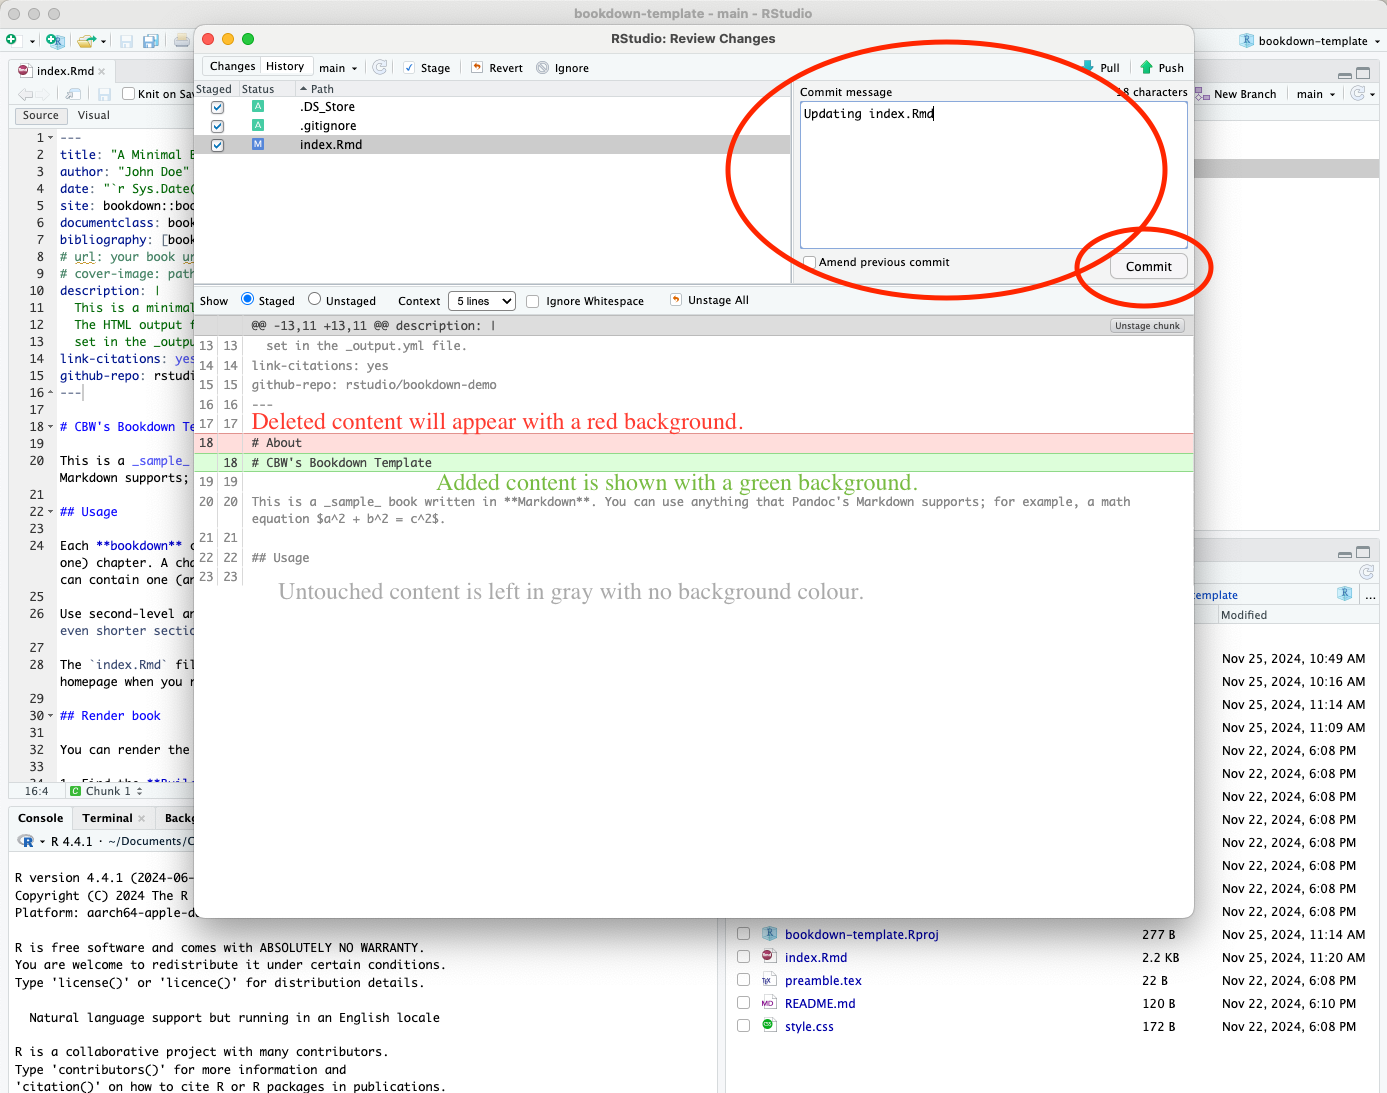
\includegraphics{img/git-instruct/git-commit-window.png}
\caption{git commit window pane}
\end{figure}

\begin{enumerate}
\def\labelenumi{\arabic{enumi}.}
\setcounter{enumi}{14}
\item
  Add a commit message in the corresponding box, and then press commit below it.
\item
  A new window will show up, detailing your updates. Close this window and then press \textbf{Push} to push your updates to GitHub.
\end{enumerate}

\begin{figure}
\centering
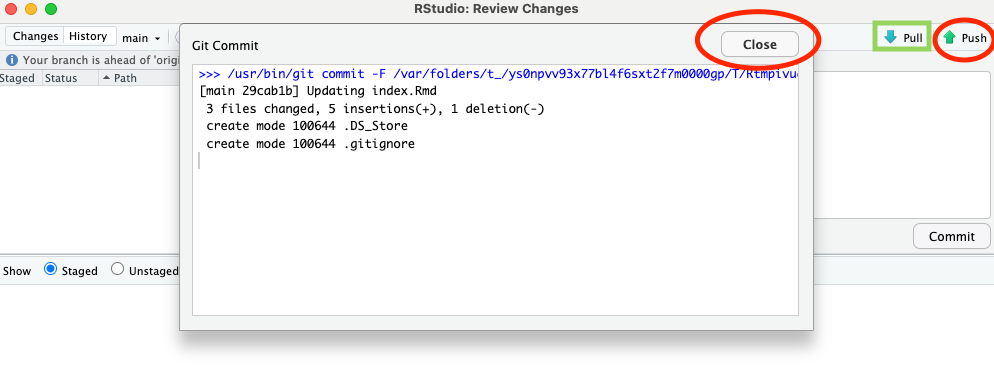
\includegraphics{img/git-instruct/git-window-post-commit.png}
\caption{post git commit window}
\end{figure}

Now, we're done! We should see the updates on GitHub now. Also note, if we ever want to pull updates from GitHub, there is also a \textbf{Pull} button in the Git window within RStudio!

\section{How to Git Clone (ISC)}\label{how-to-git-clone-isc}

\chapter{How to Deploy Your Workshop Website}\label{how-to-deploy-your-workshop-website-1}

Let's recap.

We've made a bookdown project that builds into a website. We've reconfigured the output to go to a folder called ``docs'' (output\_dir: ``docs''). We've pushed our content onto github, and also made a ``.nojekyll'' file, which we placed into docs.

Now in our ./docs folder, we have a bunch of html files that make up our website. We want GitHub to look at these files in the docs folder and host the website for us!

We deploy our website using GitHub pages. GitHub pages uses jekyll, so the .nojekyll file tells it to no longer rely on jekyll. Now, all we need to do is tell GitHub pages to deploy (create/update the website) from our docs folder.

\begin{enumerate}
\def\labelenumi{\arabic{enumi}.}
\item
  Go to your repo on GitHub.
\item
  In the top navigation bar, select settings.
  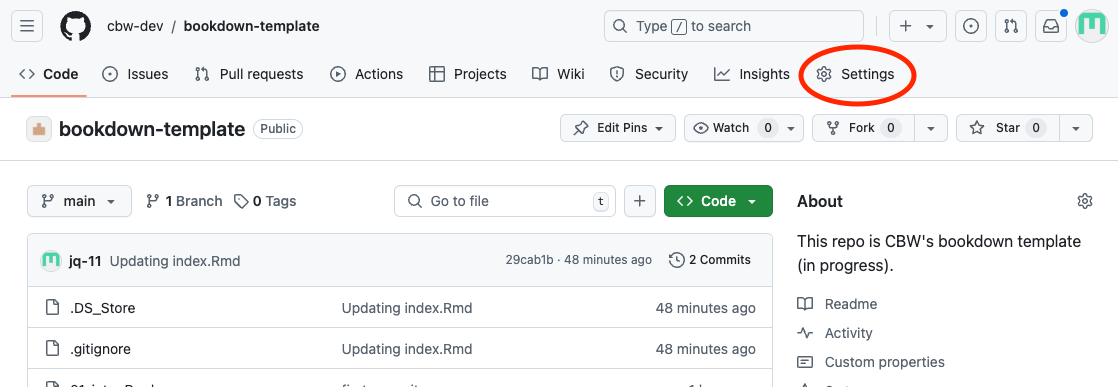
\includegraphics{img/git-instruct/github-settings.png}
\item
  Then, go to the pages sidebar.
  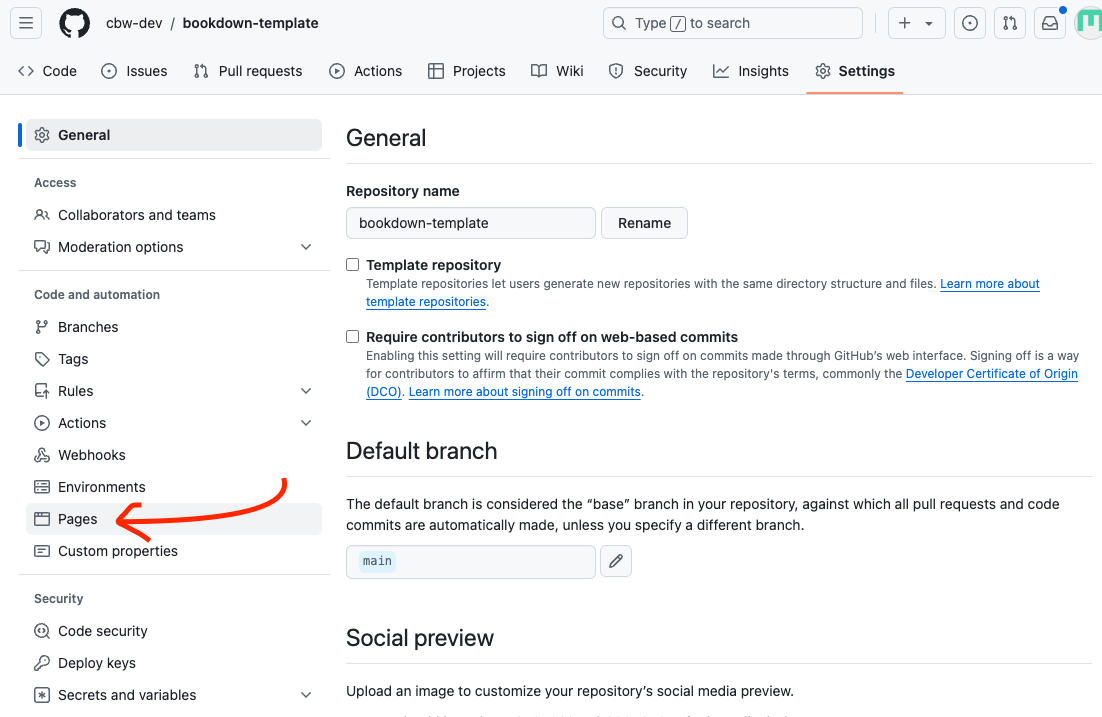
\includegraphics{img/git-instruct/github-select-pages.png}
\item
  ``Deploy from a branch'' is already selected, which is what we want. We must change the branch from ``none'' to main.
  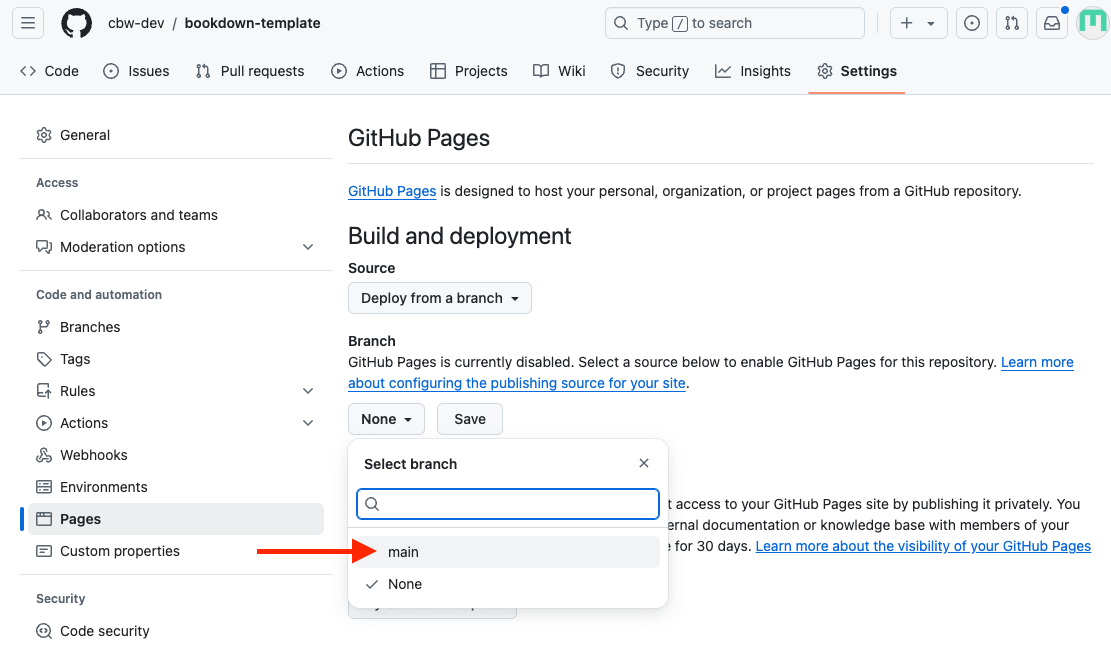
\includegraphics{img/git-instruct/github-deploy-main.png}
\item
  Then, change the folder from \texttt{/\ root} to \texttt{/docs}. Then press save.
  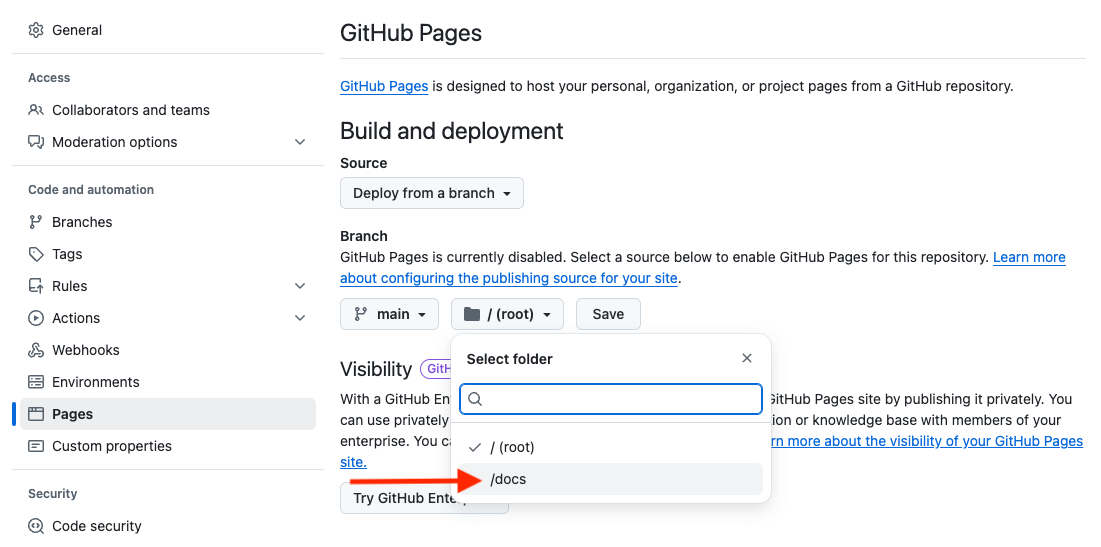
\includegraphics{img/git-instruct/github-deploy-docs.png}
\end{enumerate}

Great! Now we're waiting on the page to build and deploy, which should take less than a minute.

To see updates, go to the \textbf{Actions} page (found along the top navigation bar. This will help you understand how the deploy is working, and if it succeeded or failed.

\begin{figure}
\centering
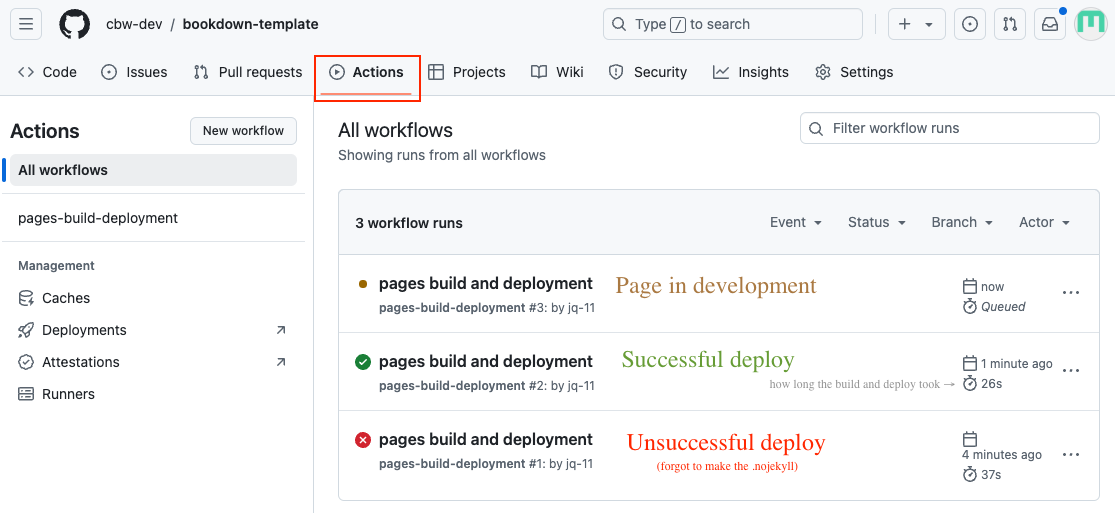
\includegraphics{img/git-instruct/github-pages-actions-explained.png}
\caption{Image showing the different possibilities of deploy a github page}
\end{figure}

You can click \textbf{pages build and deployment} for updates. It will give you errors (which may not be very clear) or the link of your deployed page!

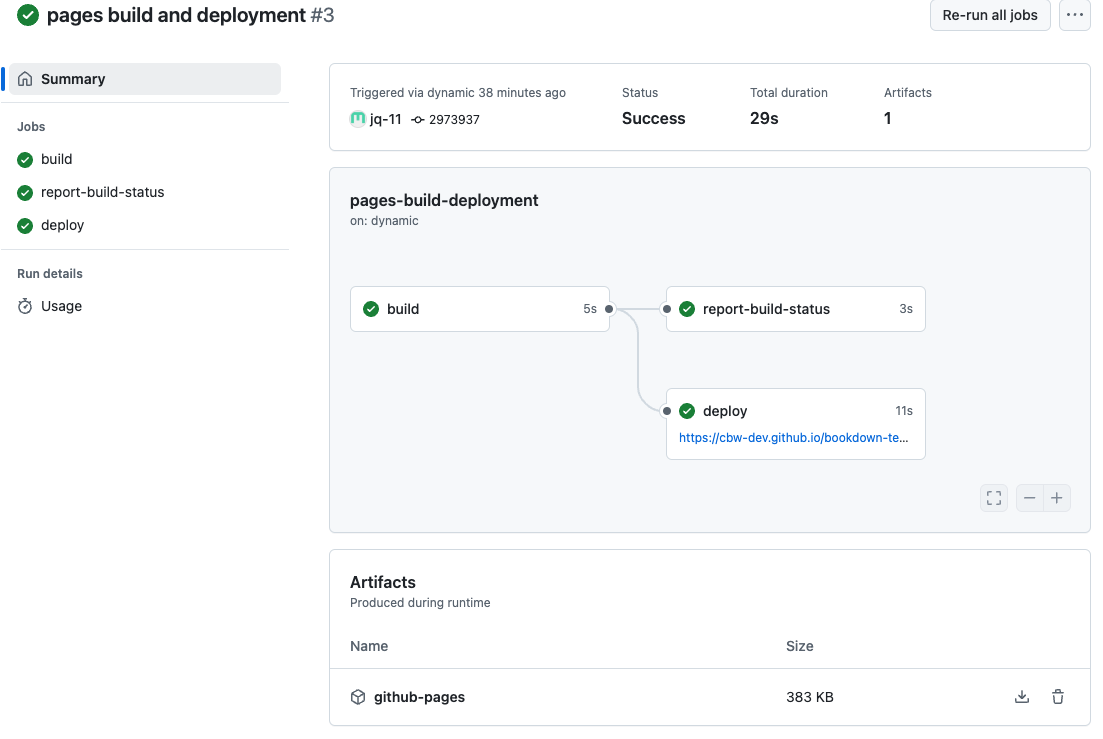
\includegraphics{img/git-instruct/successful-deploy.png}
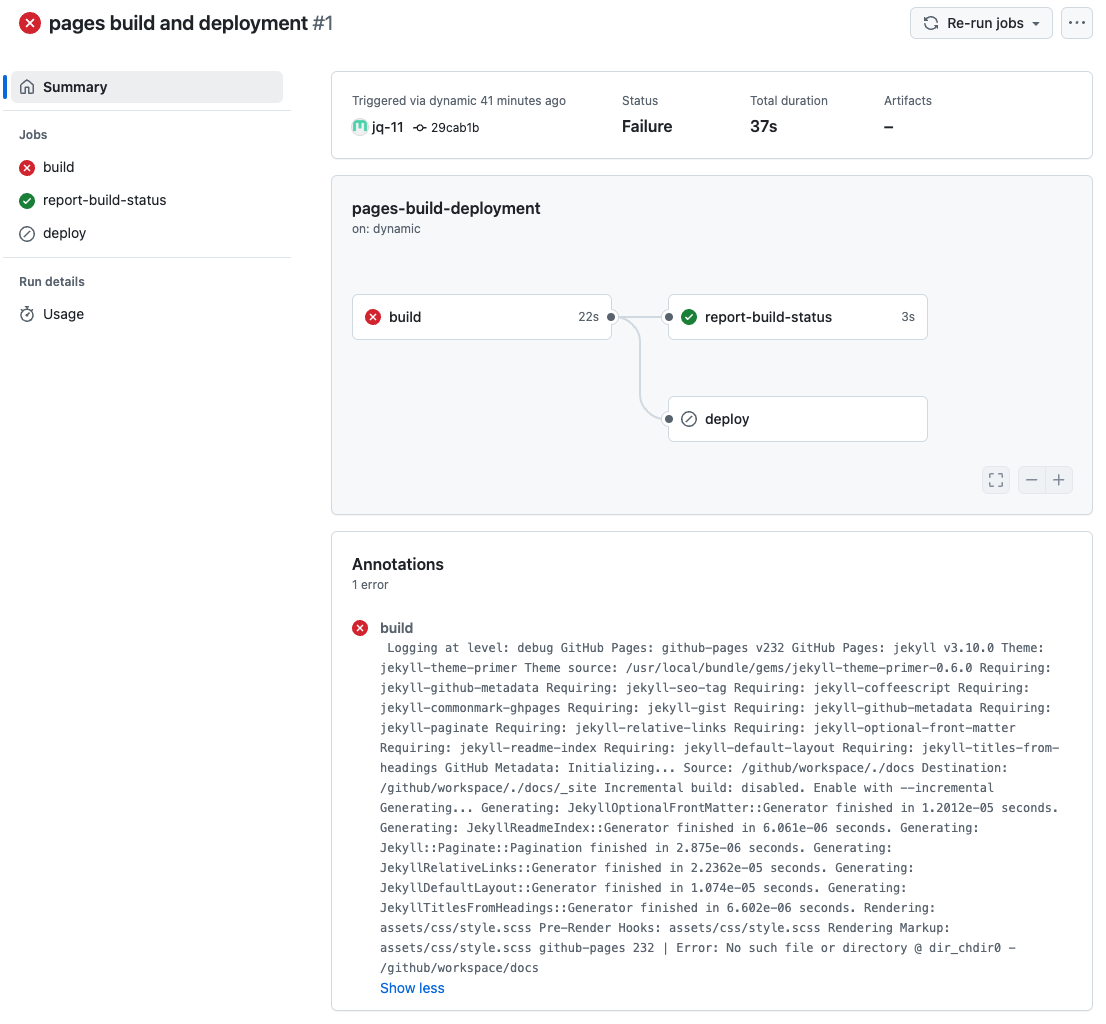
\includegraphics{img/git-instruct/failed-deploy.png}

Click around to explore more!

  \bibliography{book.bib,packages.bib}

\end{document}
